\chapter{Theory of Laser Coupled with Passive Cavity}
\label{ch:theory}
Semiconductor lasers with external cavities exhibit a variety of dynamical phenomena, depending on key parameters, comprising feedback strength, feedback delay, pump current, feedback type, and laser nonlinearity\cite{}. Among all of them the, feedback sensitivity of laser diodes is governed essentially by the feedback parameters $C$, $X$ and $\kappa_{ext}$.

In order to correct consider the feedback effect a three-mirror laser model is considered in \autoref{three_mirror_cavity}. 
% The transmission coefficent across the interface, $t_2$, includes any scattering or coupling loss, so $r_2^2+t_2^2\neq1$, in general.
\begin{figure}[ht]
    \centering
    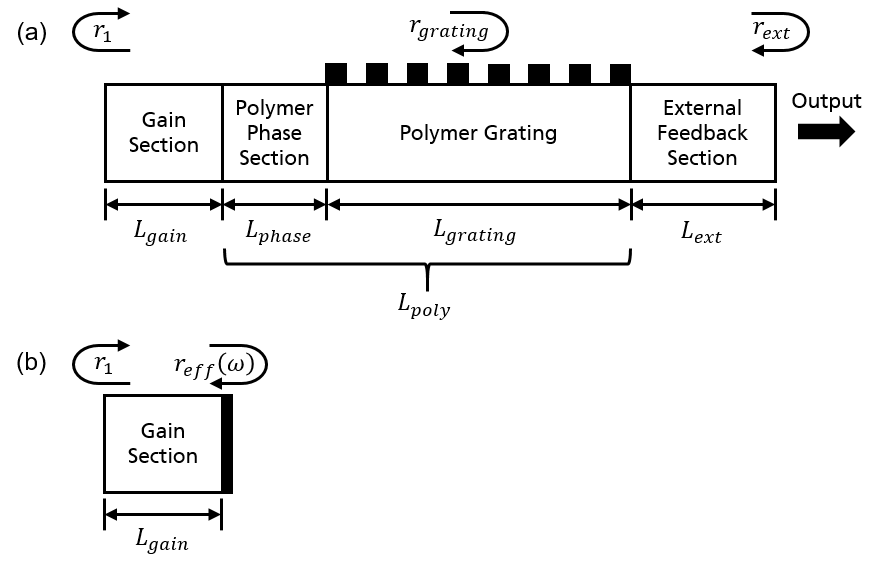
\includegraphics[width=12cm]{figures/laser_cavity_model.png}
    \caption{External cavity laser and equivalent cavity with effective mirror to model the external section.}
    \label{three_mirror_cavity}
\end{figure}

The feedback coefficient, $C$, characterizes the level of feedback in relation to how it affects the mode structure of the laser, is defined as
\begin{equation}
    C=X\sqrt{1+\alpha^2}
\end{equation}
with
\begin{equation}
    X=\frac{\tau_{ext}}{\tau_{gain}+\tau_{poly}}\kappa_{ext}
\end{equation}
\begin{equation}
    \kappa_{ext}=\frac{r_{ext}}{r_{grating}}\qty(1-\abs{r_{grating}}^2)
\end{equation}
$\kappa_{ext}$ is the coupling coefficient from the grating reflector to the external cavity.

The $C$ parameter indicates the laser stability under feedback is affected both by external reflector $r_{ext}$ and external round-time delay $\tau_{ext}$. When $C<1$, usually for weak feedback and relatively short external cavityies, the laser operates in a single mode lasing region and is phase dependent to the external feedback, when $C>1$, over one stable mode will appear and the laser will undergo a route-to-chaos behavior until it reaches coherence-collapse \cite{} region, which is the region IV for the experimentally identified five distinct regimes of laser performance under feedback \cite{tkach1986regimes}, if the feedback strength is even higher, the laser will become stable single mode again lasing with the compound cavity mode.

Rate equation models of the field and phase including the time delay of the feedback field reveal unstable solutions and chaotic behavior at these high feedback levels \cite{tkach1986regimes}. The collapse begins at the transition to regime IV, where the normally small satellite peaks created by noise-induced relaxation oscillations (depicted in Fig. 5.23) grow larger and larger, eventually becoming comparable to the central peak and broadening the linewidth dramatically \cite{coldren2012diode}.

In general, to understand the static lasing behavior under feedback is useful to consider the three-mirror cavity and by the feedback coefficient $C$, it also relates to the linewidth reduction under weak feedback condition, which will be explained in \autoref{sec:linewidth_and_chirp_reduction}. However, in order to understand the dynamic lasing behavior we can generally consider the three-mirror cavity as an equivalent two-mirror cavity (shown in \autoref{three_mirror_cavity}), which replaces the passive section by an effective mirror with reflectivity $r_{eff}$. The vale of $r_{eff}$ is defined as:
\begin{equation}
    r_{eff}=\frac{r_{grating}+r_{ext}W}{1+r_{grating}r_{ext}W}
    \label{effective_reflectivity}
\end{equation}
\begin{equation}
    W=e^{-2\alpha_{poly}L_{ext}}e^{-2i\beta_{poly}L_{ext}}
\end{equation}

The round trip phase within the laser diode cavity must be equal to an integer multiple of $2\pi$ yielding the phase condition
\begin{equation}
    2\beta L+\phi_r=2\pi m, m=integer
\end{equation}

The mode spacing in frequency is defined as:
\begin{equation}
    dv=\frac{c}{2(n_{ga}L_a+n_{gp}L_{eff})}
    \label{mode_spacing}
\end{equation}

If no reflection exists at the active-passive interface ($r_2=0$) and $r_3$ is positive and real, then $\phi_{eff}=-2\beta_pL_p$, and $L_{eff}=L_p$.



In 1980, Lang and Kobayashi published a rate equation model (the LK model) for a single-mode laser, describing the time evolution of the complex optical field and the carriers. They included the influence of the optical feedback by considering the interference of the laser field with its own coherent delayed field that had propagated once through the external cavity (Lang and Kobayashi, 1980). The model can be written as equations for the excess number of carriers $n(t)=N(t)-N_{th}$ with respect to the solitary threshold level $N_{th}$, and for the slowly varying complex electrical field amplitude $E(t)$:
\begin{equation}
    \dv{E(t)}{t}=\frac{1}{2}\qty(1+i\alpha)\xi n(t)E(t)+\kappa E\qty(t-\tau_f)e^{-i\omega_0\tau_f}
    \label{Lang_Kobayashi_1}
\end{equation}
\begin{equation}
    \dv{n(t)}{t}=\qty(p-1)\frac{I_{th}}{e}-\gamma_e n(t)-\qty[\Gamma_0+\xi n(t)]P(t)
    \label{Lang_Kobayashi_2}
\end{equation}

The optical feedback is taken into account via the feedback term at the end of \autoref{Lang_Kobayashi_1}, including $\kappa$ as the feedback rate and $\tau_f$ as the delay time. The optical field is normalized such that $P(t)=\abs{E(t)}^2$ is the photon number, $\omega_0$ represents the angular optical frequency of the solitary laser, $\xi$ is the differential gain, $\Gamma_0=1/T_p$ is the cavity decay rate, and $\gamma_e=1/T_e$ is the inverse carrier lifetime. The bias current at the solitary laser threshold is denoted as $I_{th}$, $e$ is the electron charge, $p$ is the pump parameter, and $\alpha$ is the so-called linewidth enhancement factor discussed in more detail below. The excess phase $\phi_f$ that the opitcal field accmulates within theexternal cavity can be defined as $\phi_f=\omega_0\tau_f\mod2\pi$.

\section{Linewidth and Chirp Reduction}\label{sec:linewidth_and_chirp_reduction}
Linewidth and chirp reduction due to the optical feedback is related to the same factor $F$, which is given as \cite{kazarinov1987relation}
\begin{equation}
    F=1+\frac{1}{\tau_{gain}}\dv{\phi_{r_{eff}}}{\omega}+\frac{\alpha}{\tau_{gain}}\dv{\ln{r_{eff}}}{\omega}=1+A+B
    \label{eq:F_factor}
\end{equation}
\begin{equation}
    A=\frac{1}{\tau_{gain}}\dv{\ln{r_{eff}}}{\omega}
    \label{eq:F_factor_A}
\end{equation}
\begin{equation}
    B=\frac{\alpha}{\tau_{gain}}\dv{\ln{r_{eff}}}{\omega}
    \label{eq:F_factor_B}
\end{equation}
because \autoref{eq:F_factor_A} is the freqeuncy-derivative of the $r_R$ phase, it denotes the effecitve round-trip time in the external cavity dived by $\tau_{in}$ \cite{}. That is, parameter $A$ represents the ratio of the photon numbers outside to inside the gain medium. It remains nearly constant once the laser cavity is formed. However, parameter $B$, representing the slope of the spectral reflectivity, is changed if the lasing mode is detuned. Thus, it represents the contribution of the detuned loading effect which will be explained in \autoref{sec:detuned_loading}.

If $\Delta\omega_0$ is denoted as the adiabatic chirp in the absence of feedback, then the chirp with external cavity $\Delta\omega$ is obtained as \cite{kazarinov1987relation}
\begin{equation}
    \Delta\omega=\frac{\Delta\omega_0}{F}
\end{equation}
if the spectral linewidth without external feedback is denoted by $\Delta\nu_0$, the spectral linewidth with the external cavity $\Delta\nu$ is simply obtianed as \cite{}
\begin{equation}
    \Delta\nu=\frac{\Delta\nu_0}{F^2}
\end{equation}

Consider the different feedback regions, the reduction factor at weak feedback ($C<1$) becomes
\begin{equation}
    F=1+C\cos(\phi_{ext}+\arctan\alpha)
    \label{F_weak_feedback}
\end{equation}
for strong feedback, which is more interesting and stable for the practical use, the factor $F$ becomes
\begin{equation}
    F=1+f_{ext}\frac{\tau_{ext}}{\tau_{gain}+\tau_{poly}}
    \label{F_strogn_feedback}
\end{equation}

According to this we can calculate the linewidth reduction factor $F^2$ versus the external cavity length as shown in \autoref{fig:linewidth_reduction_factor}, which will be used for the device design in \autoref{sec:design}.
\begin{figure}[ht]
    \centering
    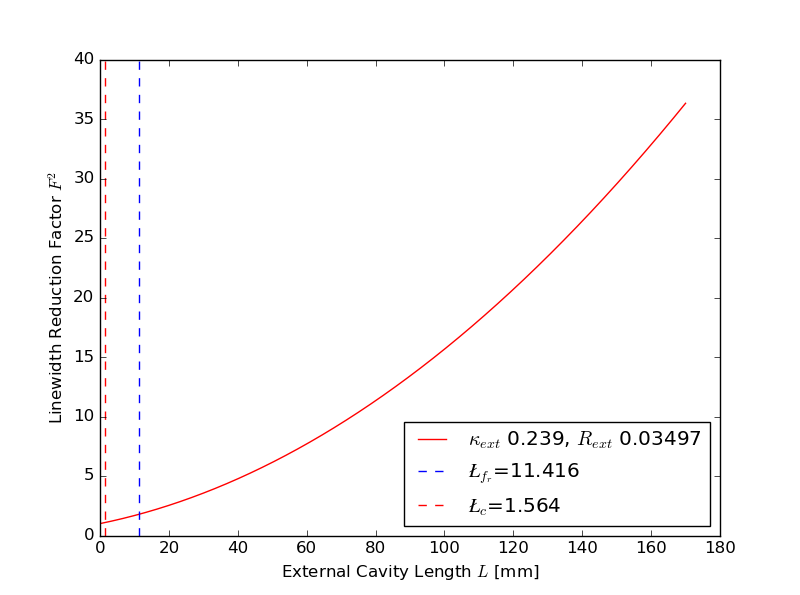
\includegraphics[width=10cm]{figures/reduction_factor.png}
    \caption{Linewidth reduction factor}
    \label{fig:linewidth_reduction_factor}
\end{figure}

\section{Bandwidth Enhancement}\label{sec:bandwidth_enhancement}
The maximum bit-rate achieved by direct modulated lasers is typically limited by the well known resonance between carriers and photons \cite{coldren2012diode}, many solutions have been proposed to overcome this restriction. Three approaches to achieve broader bandwidth are explored in detail. 

\subsection{Detuned Loading Condition}\label{subsec:detuned_loading}
The first mechanism identified to extend the modulation bandwidth of a semiconductor laser is the detuned loading effect that is due the dispersion effect introduced by a coupled cavity2,3 or by a distributed mirror (DBR4–6 or DFB7). It can be achieved when positioning the lasing mode at a slightly higher wavelength respect to the minimum threshold gain condition, which means the lasing mode of a DBR laser is oscillating at the slope of its grating response. It is reported that when the laser is operating at the longer wavelength side, the enhancement of modulation speed, reduction of phase noise (linewidth), and suppression of FM modulation (chirping) can be achieved \cite{vahala1984detuned}.
The detuned loading of the laser cavity increases the interaction between the photons and the free carriers in the laser cavity \cite{vahala1984detuned} which will both increase the modulation bandwidth and reduce the variation of the carrier density during modulation \cite{kjebon2002experimental}. 

\begin{figure}[ht]
    \centering
    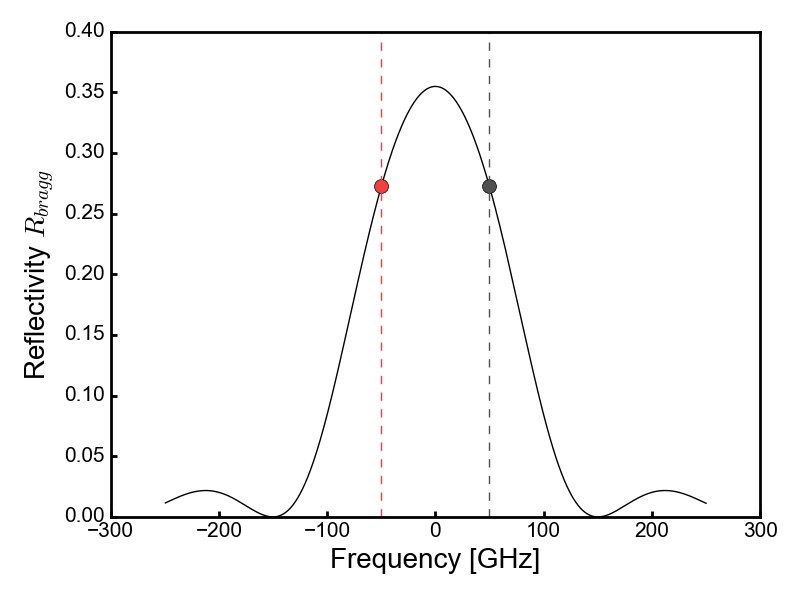
\includegraphics[width=.65\linewidth]{figures/detuned_loading_principle.png}
    \caption{Detuned loading condition with respect to the grating response. The red and grey dots correspond to the lasing mode detuend to the longer and shorter wavelength sides.}
    \label{fig:detuned_loading_principle}
\end{figure}


% \begin{figure}[!htb]
%   \begin{minipage}{0.48\textwidth}
%      \centering
%      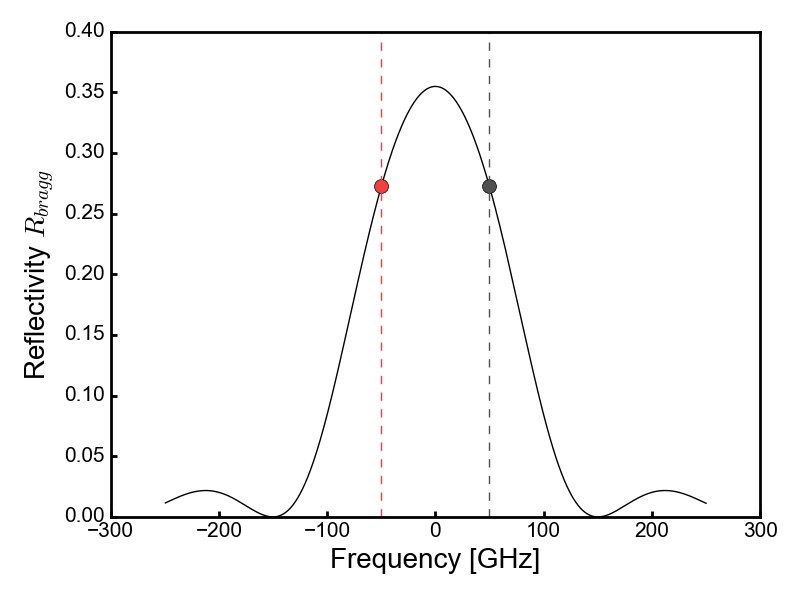
\includegraphics[width=.7\linewidth]{figures/detuned_loading_principle.png}
%      \caption{Detuned loading operation principle}
%      \label{fig:detuned_loading_principle}
%   \end{minipage}\hfill
%   \begin{minipage}{0.48\textwidth}
%      \centering
%      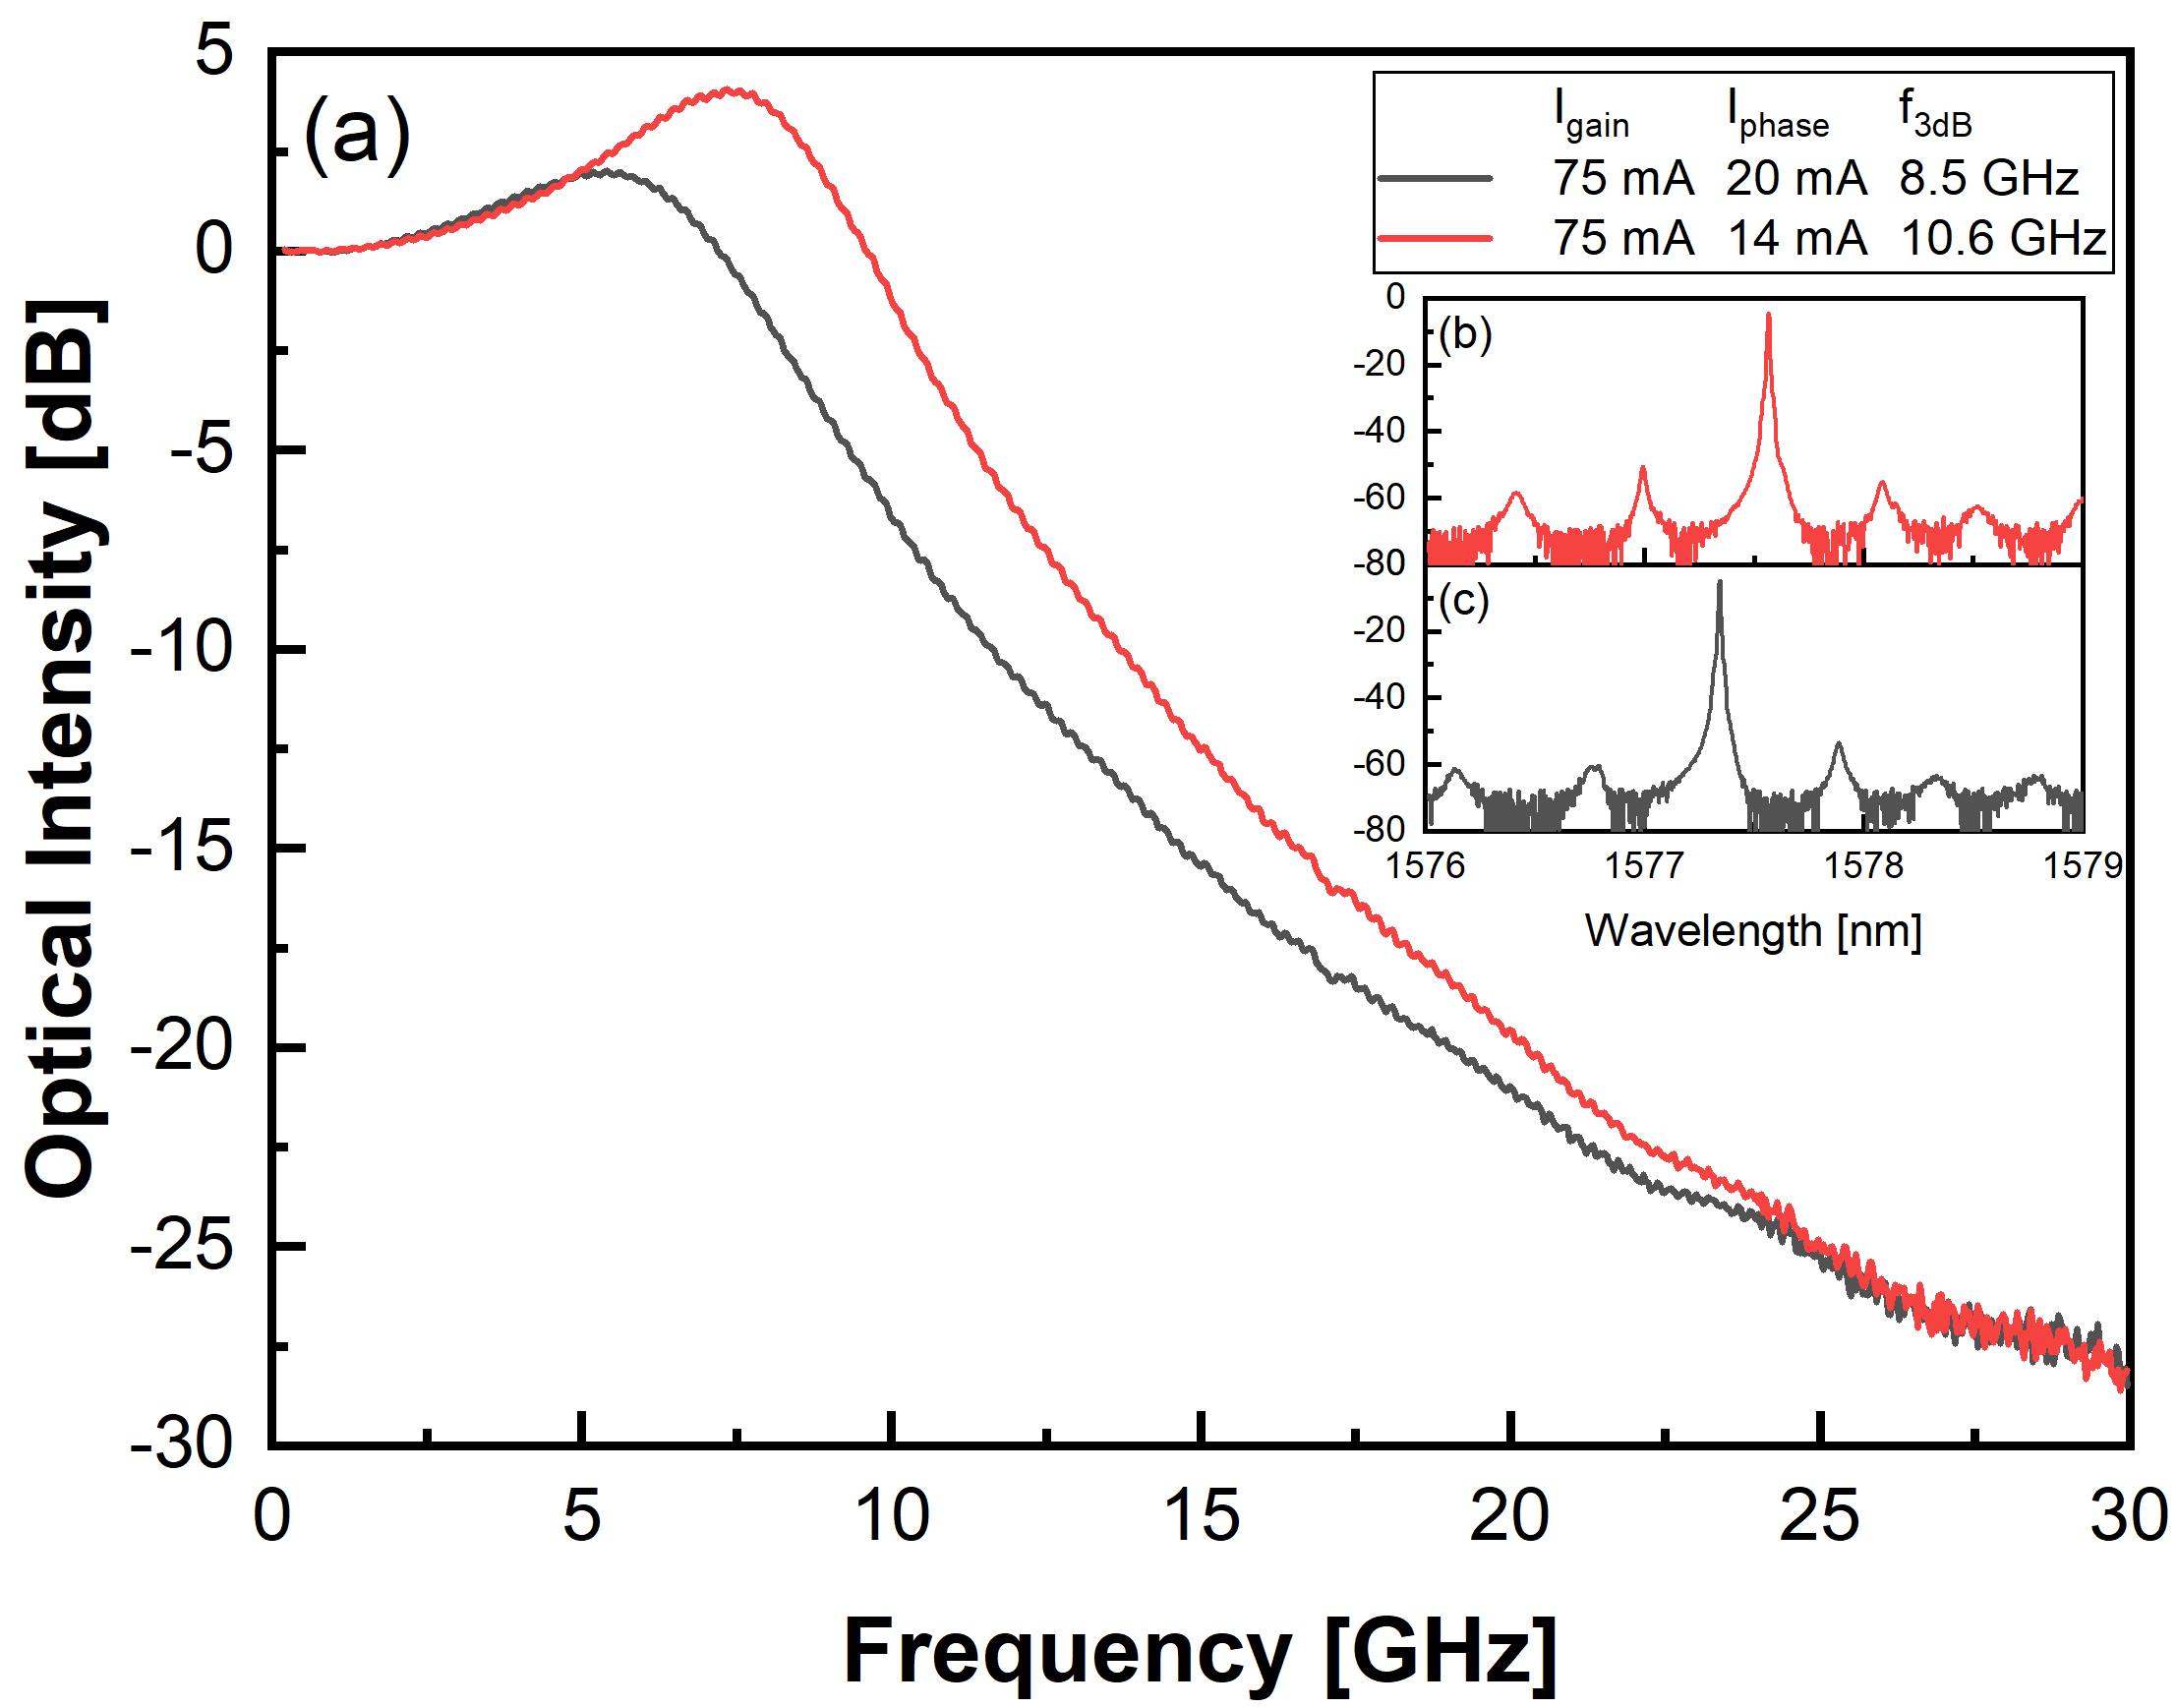
\includegraphics[width=.7\linewidth]{figures/detuned_loading.png}
%      \caption{Laser under detuned loading condition}
%      \label{fig:detuned_loading}
%   \end{minipage}
% \end{figure}

Operating our DBR laser under the detuned loading condition was measured and the result is shown in \autoref{fig:detuned_loading}. When the laser is lasing on the slope of the grating response, the side modes have a different gain spectrum relative to the peak of the grating response, which introduces the asymmetric behavior of the side modes. In this case, when the left side mode is higher than the right one, means the lasing mode is operating at the longer wavelength side of the grating response, and vice versa.

\subsection{Undamped Relaxation Oscillation}\label{subsec:undamped_RO}
Relaxation oscillation in a semiconductor laser occurs because the carrier cannot follow the photon decay rate, it usually smoothly decays out as long as the disturbance (e.g. external feedback) is small enough \cite{ohtsubo2012semiconductor}. However, it can become undamped when the laser exhibits the feedback from the chip facet, which even influences the optical spectra that the undamping peaks are appearing beside the main mode with the mode spacing of relaxation frequency (typically 1\textasciitilde{}10 GHz). The undamped relaxation oscillation occurs for the appropriate combinations of feedback phase and strength as shown in \autoref{fig:undamped_RO_phase_scan}. The satellite peaks first appear as \autoref{fig:undamped_RO} (b) and then slowly increase their intensity and move towards the main peak, follows with more satellite peaks appearing when the corresponding relaxation oscillation frequency is decreasing. The mode spacing between the main mode and side mode in \autoref{fig:undamped_RO} (b) is 11 GHz and decreases to 9 GHz in \autoref{fig:undamped_RO} (a).
\begin{figure}[ht]
    \centering
    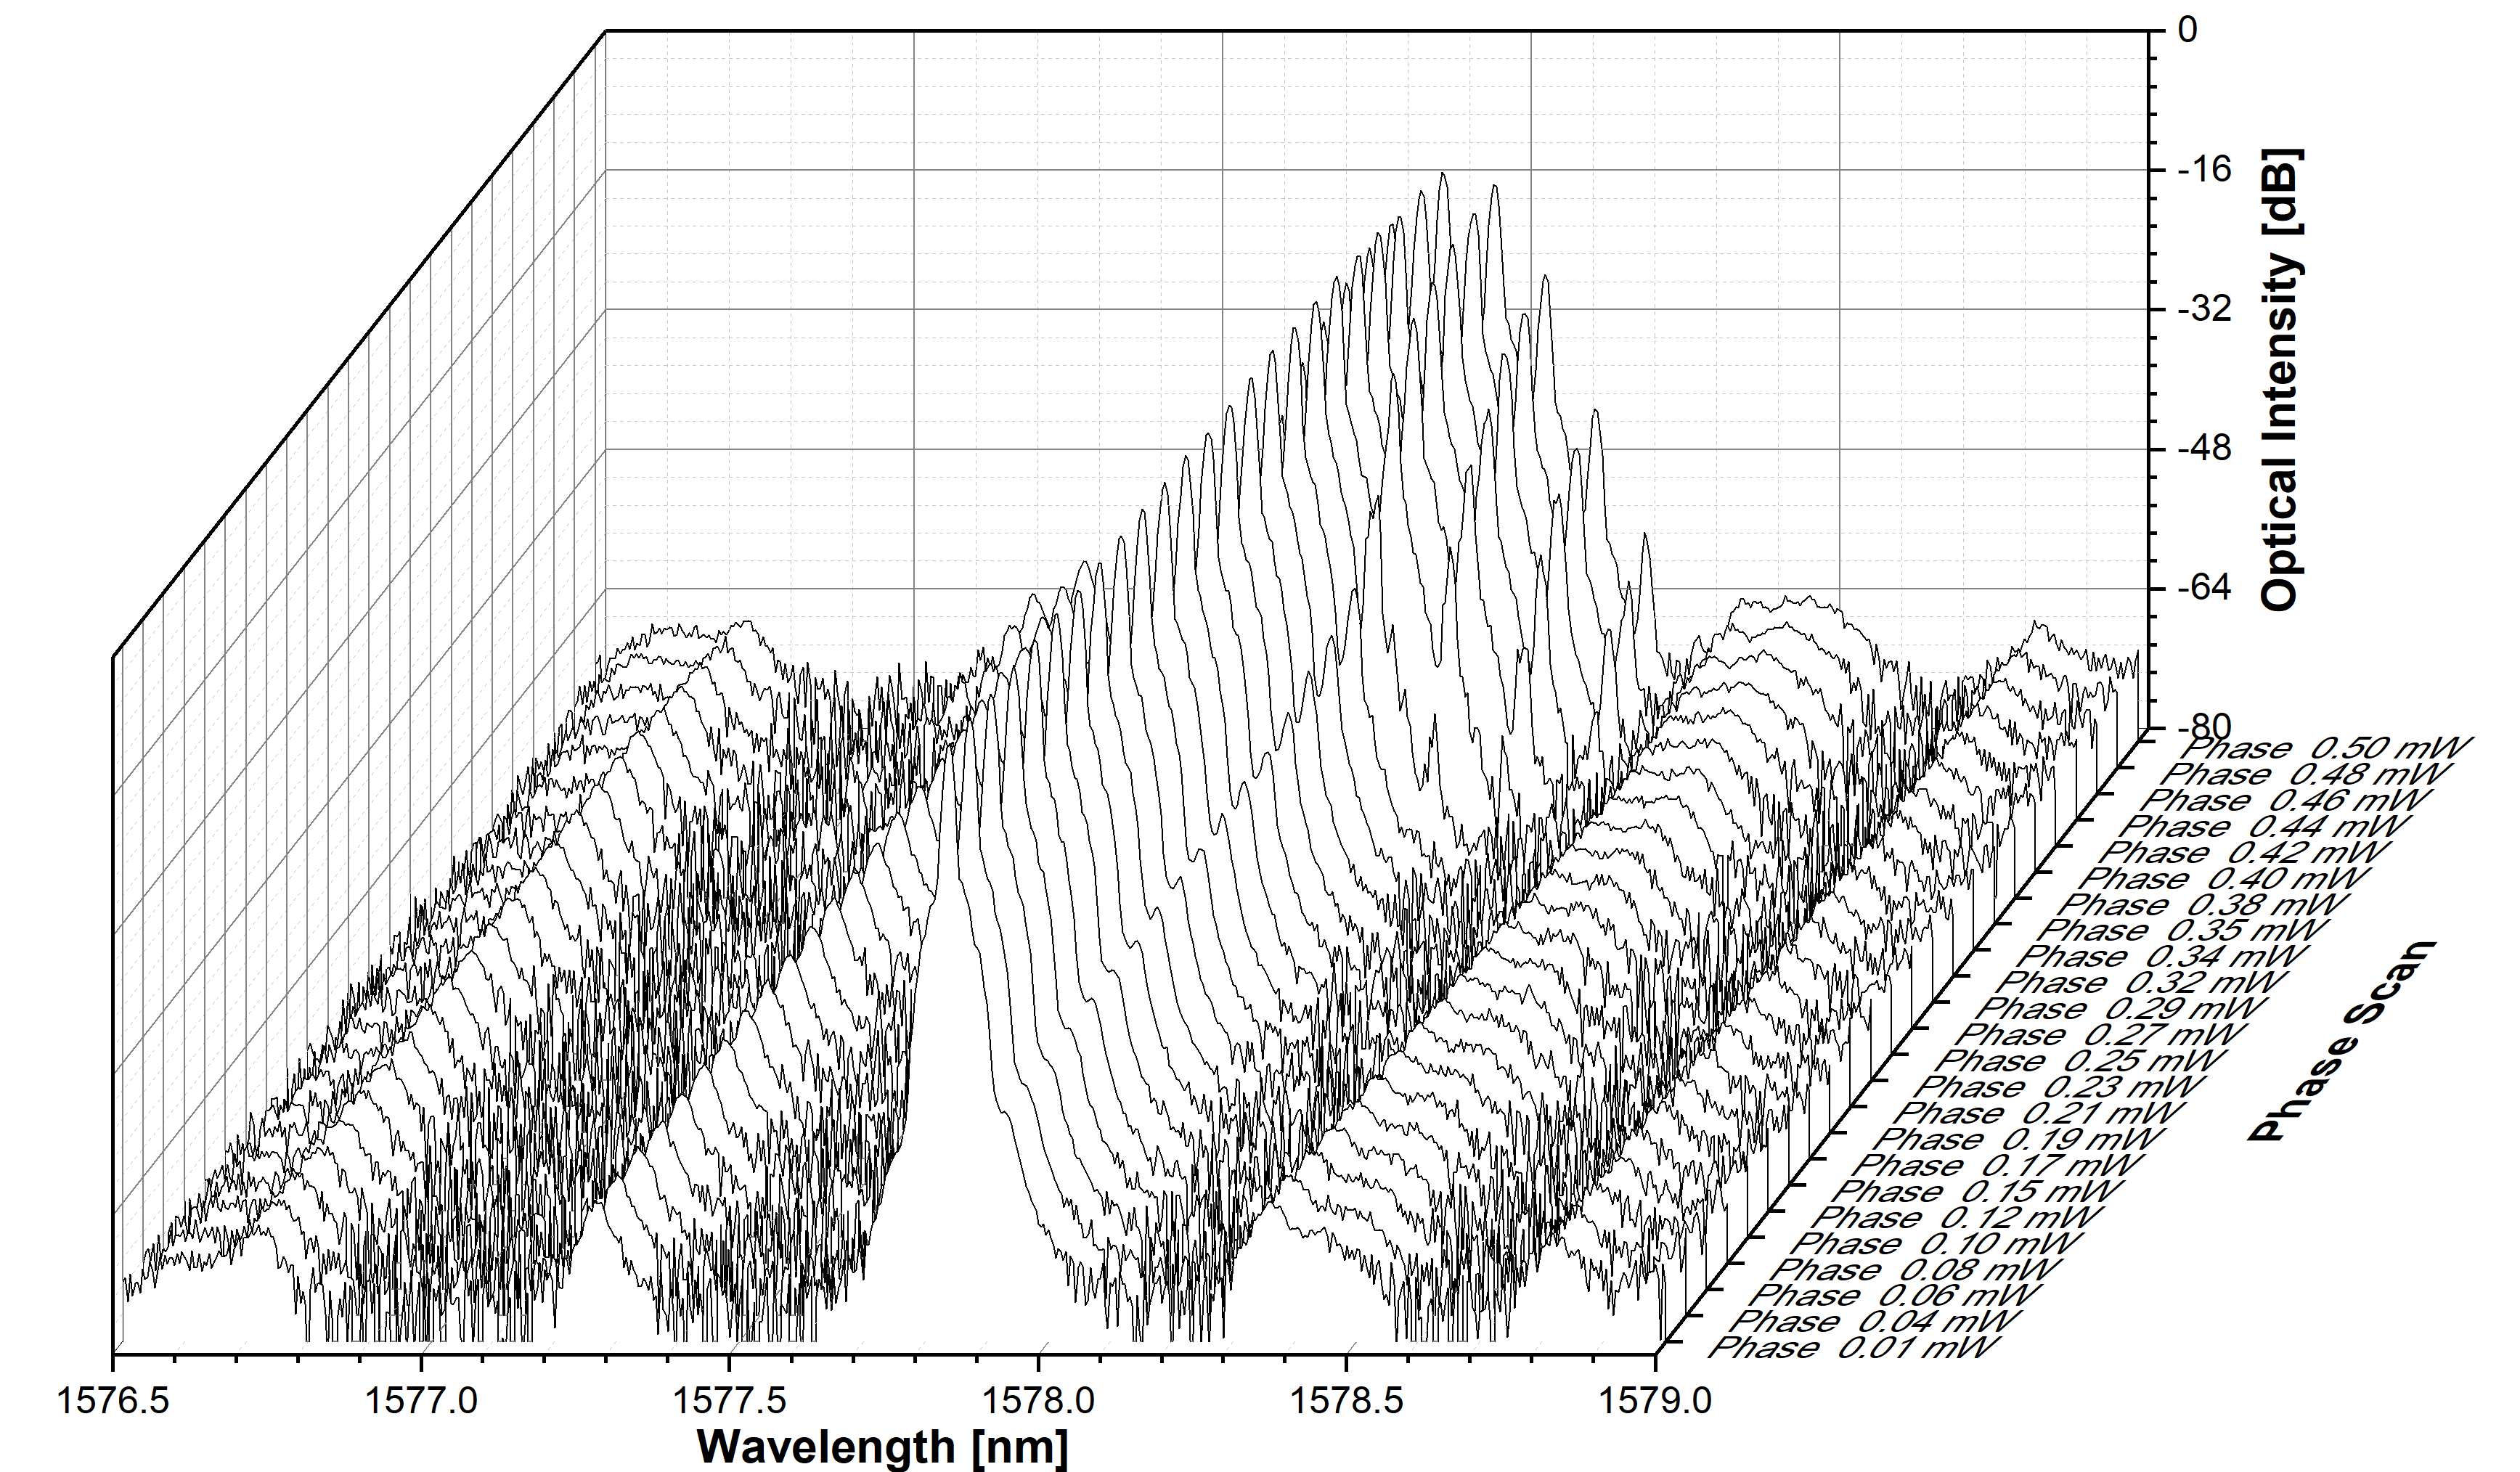
\includegraphics[width=.8\linewidth]{figures/Undamped_RO_phase_scan_grating_4621.png}
    \caption{Phase scan of the tunable laser spectra with feedback from chip facet. The side peaks of undamped RO start to appear with increasing of their intensity and shifting towards the main peak. While the applied phase current keep changing, more peaks due to undamped RO starts to appear until the laser shift to another mode and becomes stable single mode lasing again.}
    \label{fig:undamped_RO_phase_scan}
\end{figure}



Since the incoming feedback acts like a perturbation for the normal laser which introduces the amplitude modulation, the undamped RO can be also called as self-modulation or self-pulsation. The mechanism of self-pulsation is analysed and discussed in \cite{bandelow1993theory} as "dispersive Q-switching". In order to explain the self-pulsations one usually assumes some kind of a Q-switching process, where the term Q-switching denotes a switching of the quality-factor of the laser cavity. If, due to some reason to be discussed later, an increase of optical power yields a decrease of optical loss (or an increase of optical gain) within the laser, the round trip gain G may become larger than unity, yielding an exponential increase of optical power, corresponding to the rising edge of a developing pulse. On the other hand an increased power yields an increasing consumption of carriers so that finally the carrier density is too low to maintain a unity roundtrip gain and therefore the optical power collapses. A recovery time is required in order to increase the carrier density again until the next pulse develops. The repetition frequency for these pulses is of the same order as the relaxation resonance frequency \cite{petermann2012laser}.

\subsection{Photon-Photon Resonance}\label{subsec:pp_resonance}
Another approach used to extend the dynamic properties of an integrated laser is similar to detuned loading condition but in addition it takes advantage of the interaction between the lasing mode and an adjacent longitudinal cavity mode, properly separated in frequency in such a way they can interact due to the carrier pulsation introduced by the applied modulation signal at the gain section electrode. This interaction introduces a resonance in the impulse modulation (IM) response at the frequency corresponding to the modes separation. This resonance is frequently called Photon-Photon resonance (PPR), to distinguish this interaction mechanism respect to the Carrier-Photon resonance (CPR) \cite{montrosset2014laser}. The appearing of the PPR should not be too far away from the relaxation oscillation frequency so that the dip in between two peaks will not be deep enough to reach the -3 dB limation in the modulation response as shown in \autoref{fig:PP_resonance_in_modulation_response}.
\begin{figure}[ht]
    \centering
    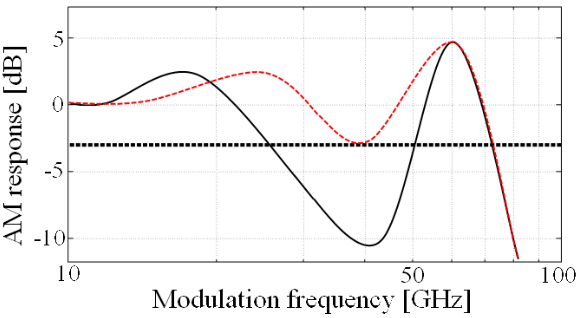
\includegraphics[width=.6\linewidth]{figures/PP_resonance_in_modulation_response.png}
    \caption{Example of modulation responses obtained in cavity exploiting the PPR effect. The black line indicates a case in which the CP and the Photon–Photon peaks are too much separated whereas in the case indicated by the red line the modulation bandwidth extension is achieved \cite{montrosset2014laser}.}
    \label{fig:PP_resonance_in_modulation_response}
\end{figure}

Here we will illustrate the operation principle using the same device parameter provided in \cite{montrosset2014laser}, which is shown in [].
\begin{figure}[ht]
    \centering
    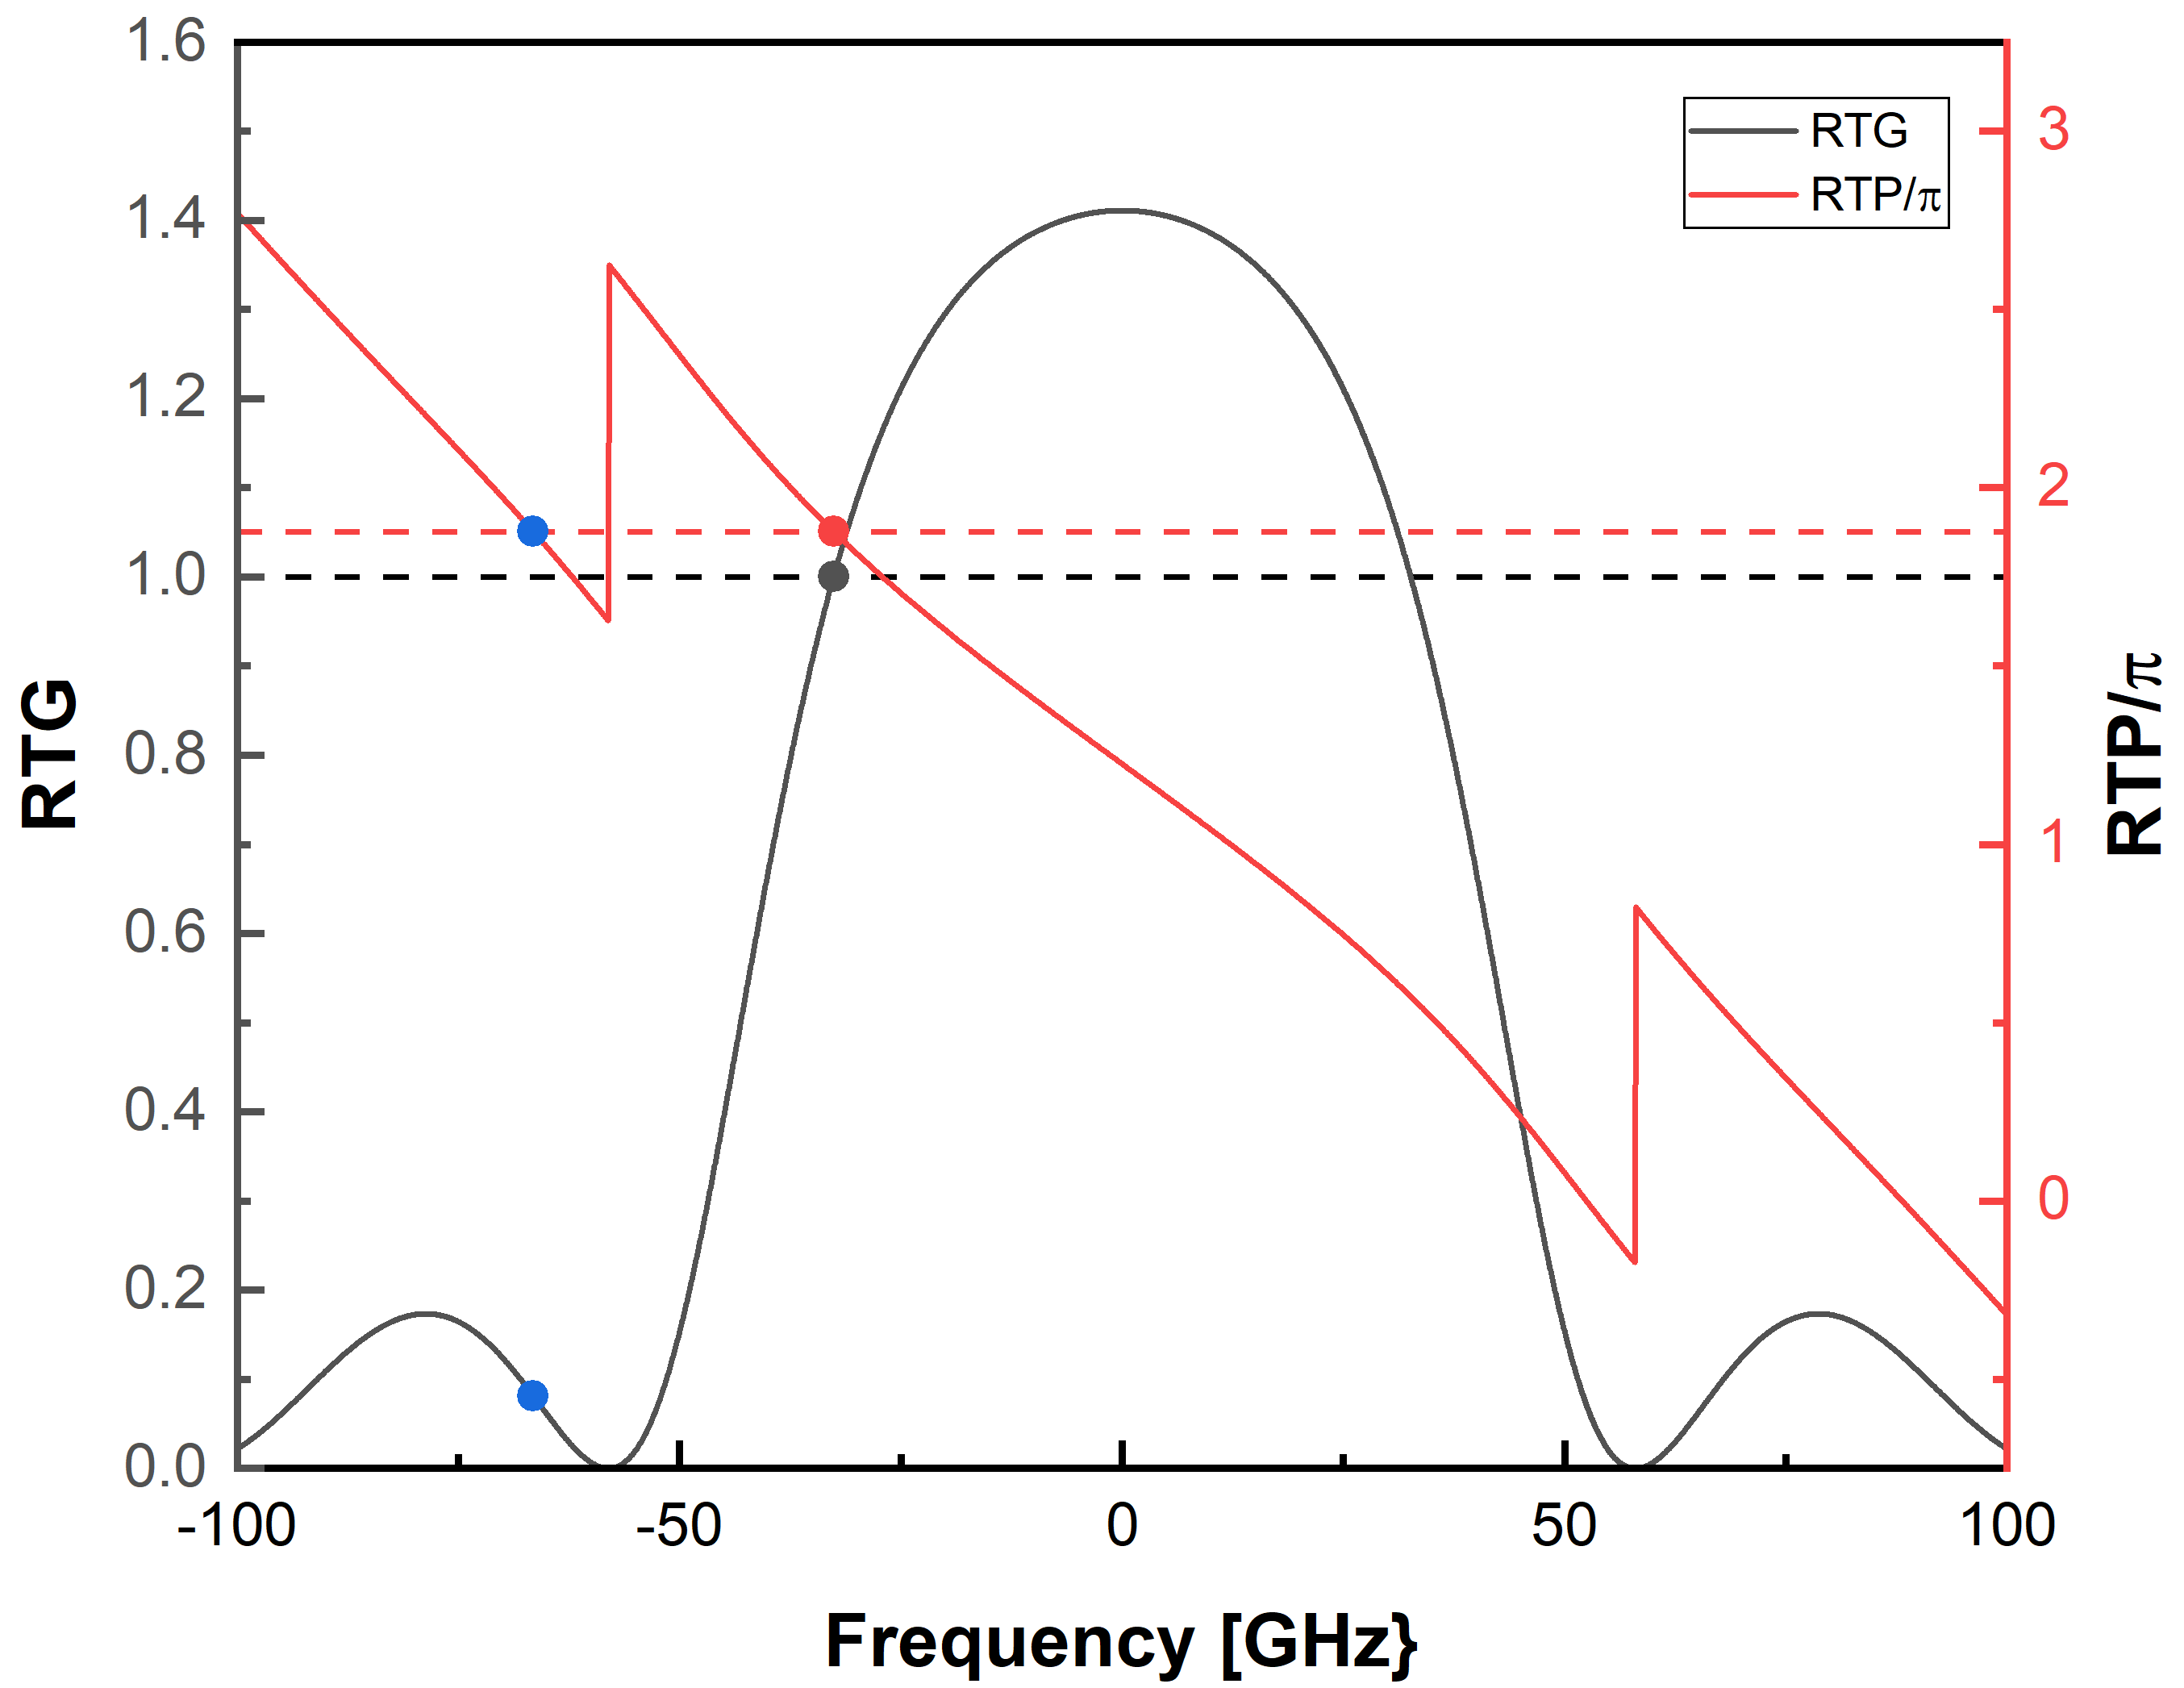
\includegraphics[width=.6\linewidth]{figures/PP_resonance_operation_principle.png}
    \caption{Photon-photon resonance adapt from \cite{montrosset2014laser}}
    \label{fig:PP_resonance_operation_principle}
\end{figure}

The most favorable operation condition is when the lasing mode $\lambda_0$ operates in the detuned loaidng condition $\lambda_0>\lambda_B$, the closest mode on other side respect to the Bragg wavelength $\lambda_1$ is strongly suppressed, and, finally, a mode on the same side respect to the Bragg wavelength $\lambda_{-1}$ is placed on the the first lobe of the Round Trip Gain (RTG) curve. In this mode configuration, the PPR effect can arise due to the coupling between mode $\lambda_0$ and $\lambda_{-1}$ \cite{montrosset2014laser}. In order to generate an adjacent longitudinal cavity mode under feedback, a strong feedback condition is required, which will form compound cavity modes with the mode spacing of the the normal cavity plus the external cavity.
% The mode spacing in frequency is defined as:
\begin{equation}
    dv=\frac{c}{2(n_{ga}L_a+n_{gp}L_{eff})}
    \label{mode_spacing}
\end{equation}

\chapter{Tunable Laser with Reflection from Chip Facet}\label{ch:normal_laser}
Characterization of the laser linewidth, RIN, bandwidth, $\alpha$ parameter and phase noise are measured with 1) Cleaved fiber with oil and 2) Lensed fiber, which corresponding to the laser without feedback and with feedback conditions. Principle of each measurement will be introduced and the results will be compared in the following sections.

\section{Linewidth Measurement}\label{sec:linewidth_measurement}
Laser linewidth is measured by self-homodyning method in the characterization. Self-homodyning can be described mathematically as a single-delay autocorrelation. The optical spectrum at $f_0$ autocorrelates with the delayed version of itself to produce a time-fluctuating spectrum, whose detected voltage has a power spectrum centered at zero frequency. For the case of a laser with Lorentzian lineshape, the half-width of the detected spectrum is equal to the linewidth of the laser.
\begin{figure}[ht]
    \centering
    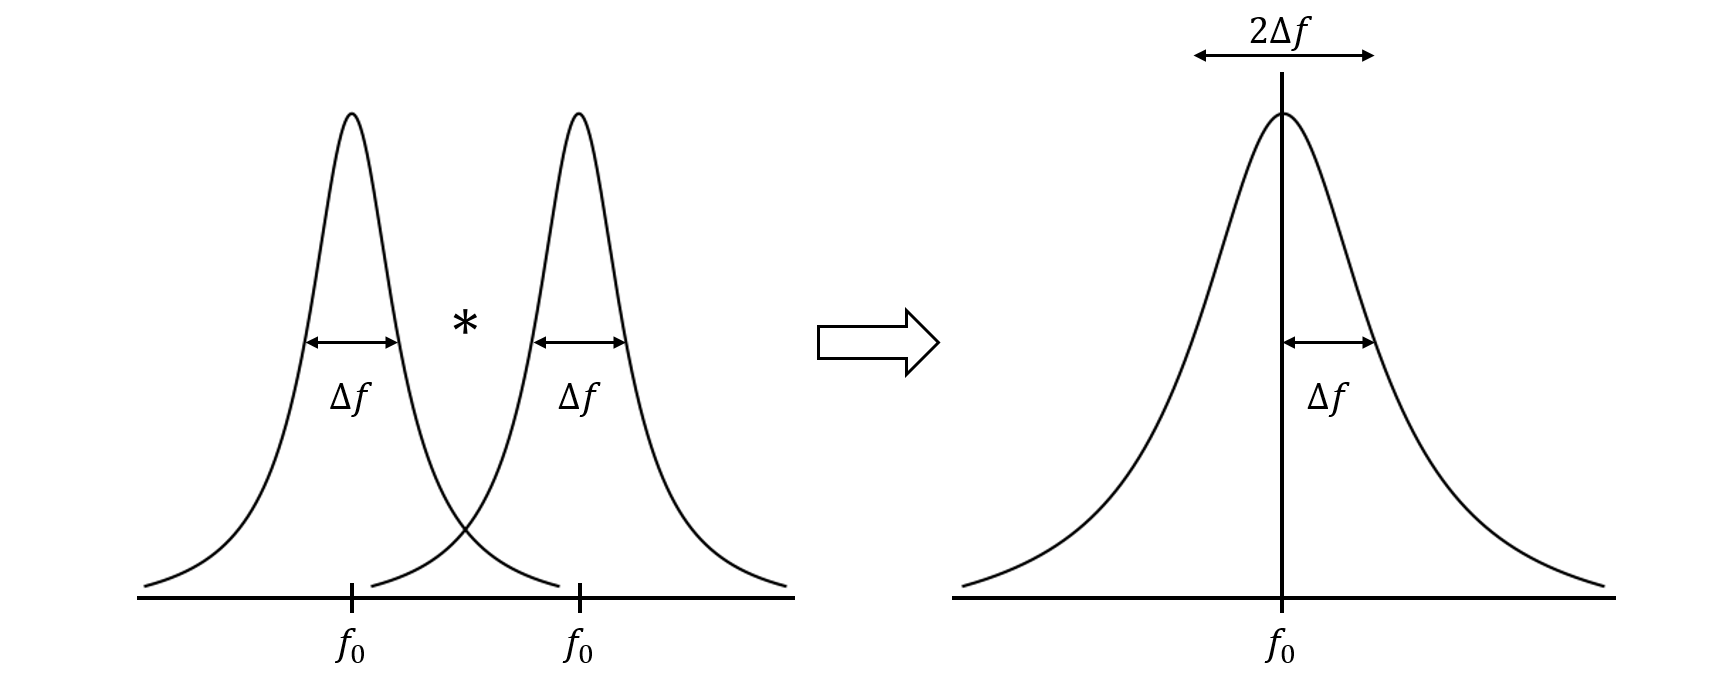
\includegraphics[width=.7\linewidth]{figures/self-homodyne.png}
    \caption{Linewidth of a DBR laser using the self-homodyne technique}
    \label{self-homodyne}
\end{figure}

The input directional coupler of the interferometer splits the light from the laser into two paths. One path is delayed in order to decorrelate the combinning signals, $P_1$ and $P_2$. The output coupler combines the two signals, which are then mixed at the photodectector of the lightwave signal analyzer.  The homodyne power spectrum is then observed on the analyzer from which the Lorentzian linewidth is measured by placing a marker at the half power frequency.
\begin{figure}[ht]
    \centering
    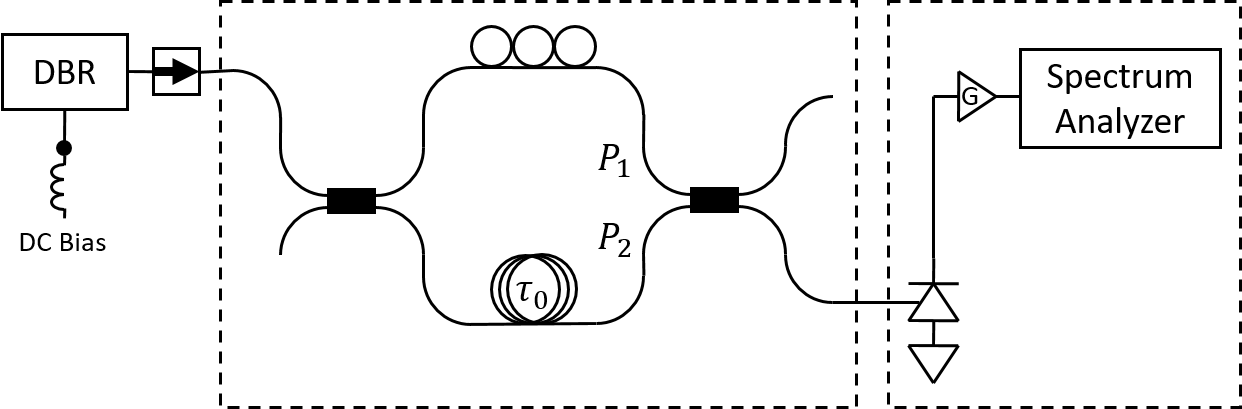
\includegraphics[width=.7\linewidth]{figures/self-homodyne_setup.png}
    \caption{Self-homodyne technique set-up}
    \label{self-homodyne_setup}
\end{figure}

\begin{figure}[ht]
    \centering
    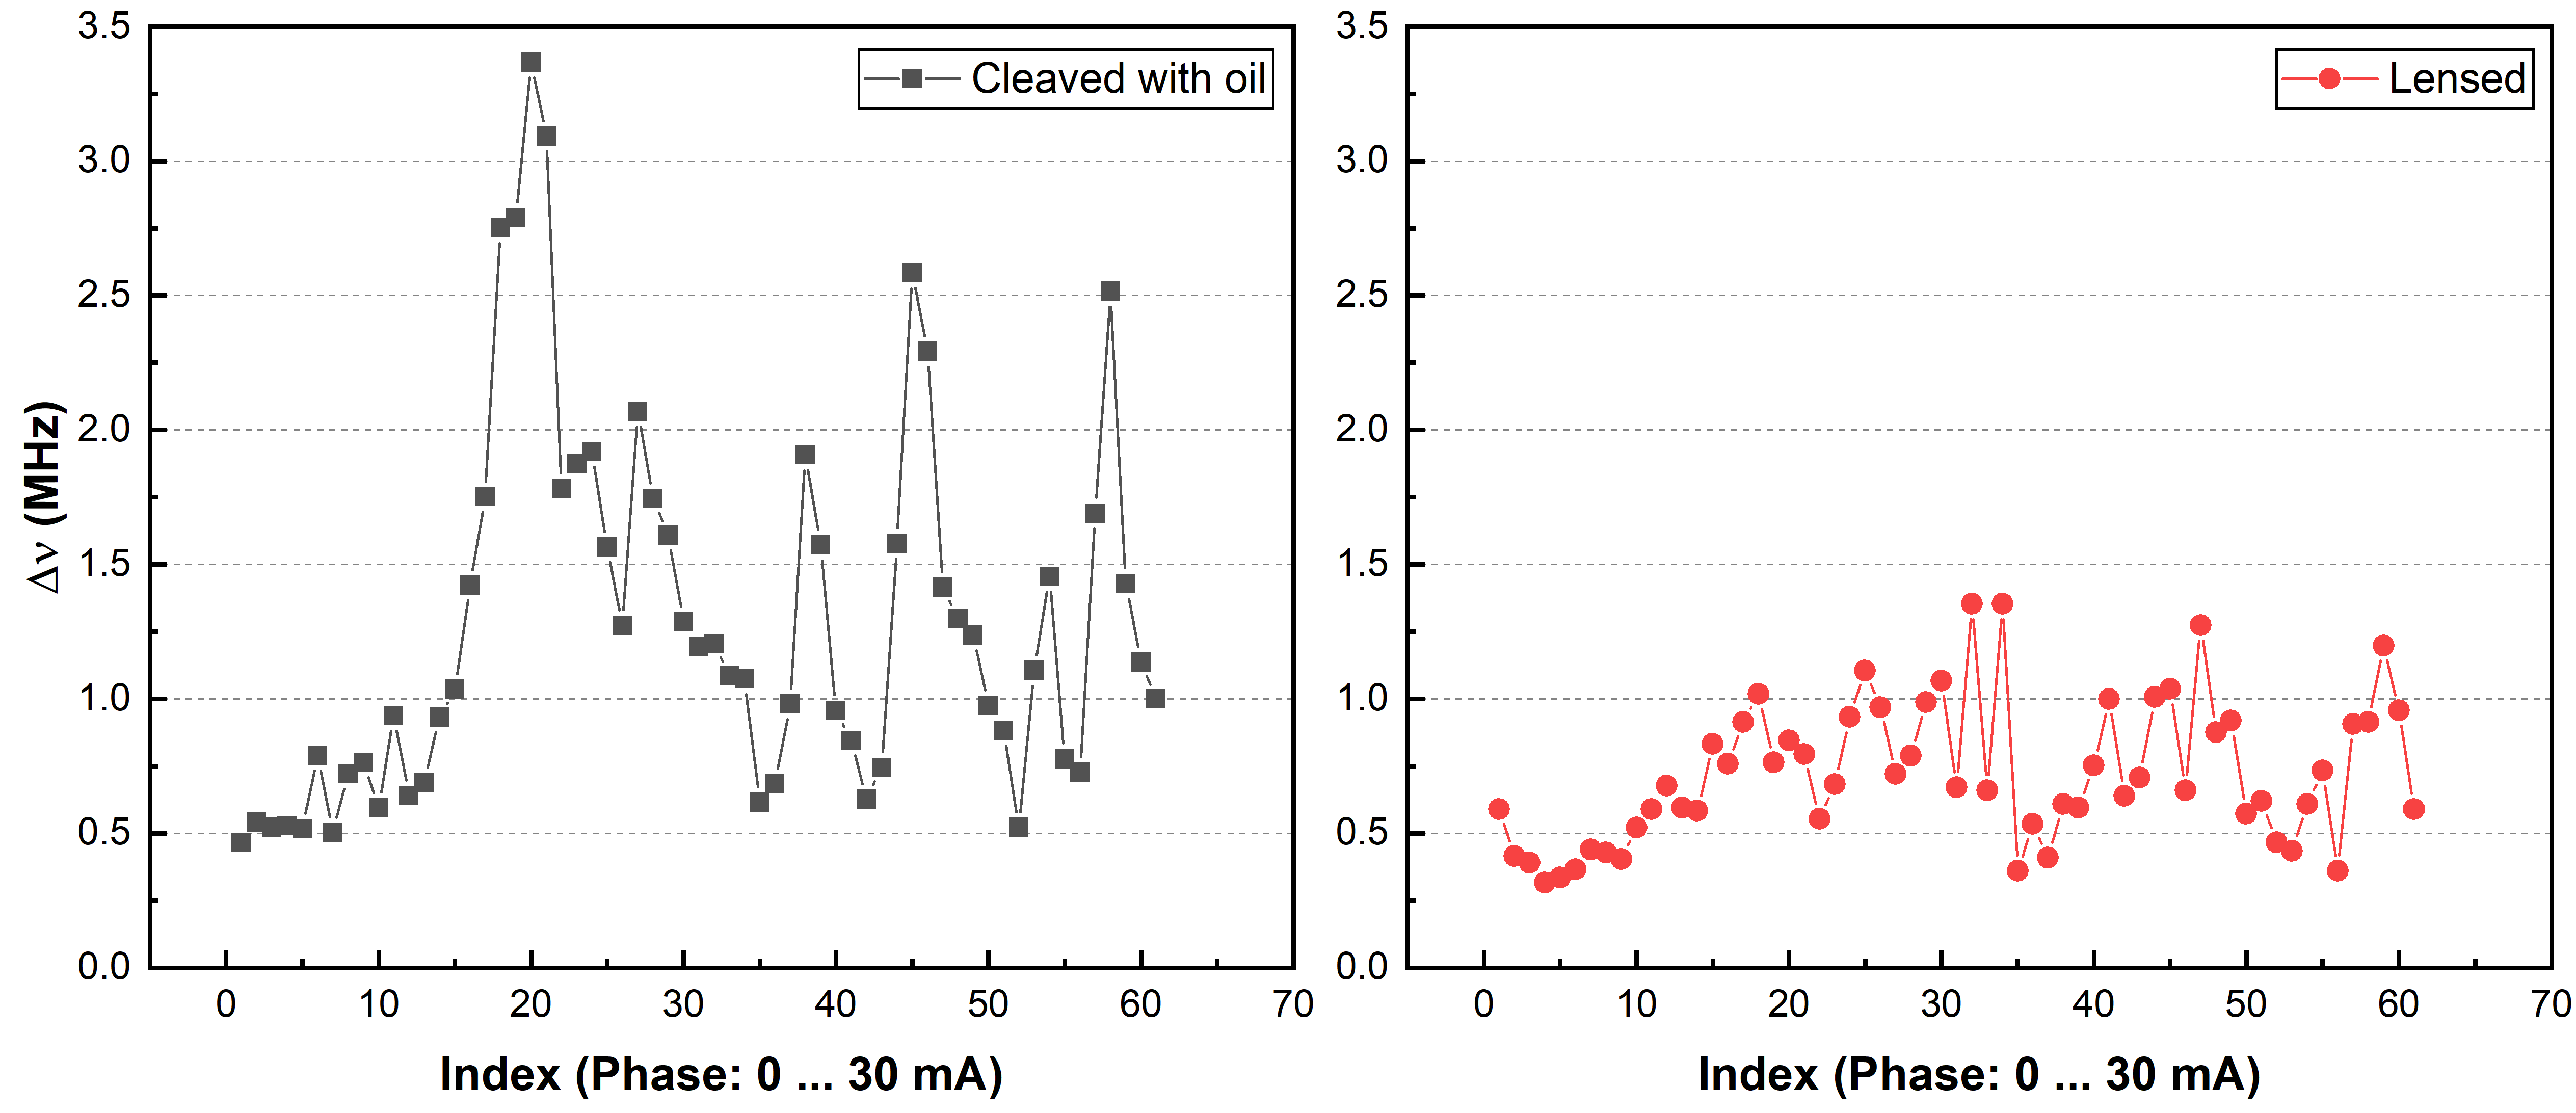
\includegraphics[width=\linewidth]{figures/LB_Cleaved_and_Lensed.png}
    \caption{Comparison of laser linewidth w/ and wo/ feedback}
    \label{fig:LB_Cleaved_and_Lensed}
\end{figure}

\section{Relative Intensity Noise (RIN) Measurement}\label{sec:RIN_measurement}
The measurement of relative intensity noise ($RIN$) describes the laser’s maximum available range for signal modulation and serves as a quality indicator of laser devices. $RIN$ is defined as the ratio of the mean-square optical intensity noise to the square of the average optical power: [cite]
\begin{equation}
    RIN=\frac{\langle \Delta P \rangle ^2}{\langle P \rangle ^2}dB/Hz
\label{RIN_1}
\end{equation}
where $\langle \Delta P \rangle ^2$ is the mean-square optical intensity fluctuations (in a 1-Hz bandwidth) at a specified frequency, and $\langle P \rangle$ is the mean optical power.

In order to measure the $RIN$, the optical power is converted to a current after the receiving photodiode and the ratio of optical powers squared is equivalent to the ratio of the detected electrical powers. Thus, $RIN$ can be expressed in terms of detected electrical powers. \autoref{RIN_1} can be rewritten as:
\begin{equation}
    RIN=\frac{N_{elec}}{P_{avg}(elec)} \ dB/Hz
    \label{RIN_2}
\end{equation}
where $N_{elec}$ is the power-spectral density of the photocurrent at a specified frequency, and $P_{avg}(elec)$ is the average power of the photocurrent.

The noise at the receiver output results from three fundamental contributions: laser intensity noise primarily due to spontaneous light emissions; thermal noise from the electronics; and photonic shot noise. Since the photonic shot noise and the receiver thermal noise are not included in the definition of $N_{elec}$, they have to be subtracted from the measured $RIN$ results:
\begin{equation}
    N_{laser}=N_{elec}-N_{shot}-N_{thermal} \ W/Hz
    \label{RIN_3}
\end{equation}
By using \autoref{RIN_2} and \autoref{RIN_3}, the value of $RIN_{laser}$ can be determined:
\begin{equation}
    RIN_{laser}=RIN(measured)-\frac{2e}{I_{avg}}-\frac{N_{thermal}}{P_{avg}(elec)}
\end{equation}
where $e$ is the elementary charge, $I_{avg}$ denotes the detected average photocurrent, $N_{thermal}$ is the measured noise floor of the lightwave signal analyzer in a 1-Hz bandwidth.
\begin{figure}[ht]
    \centering
    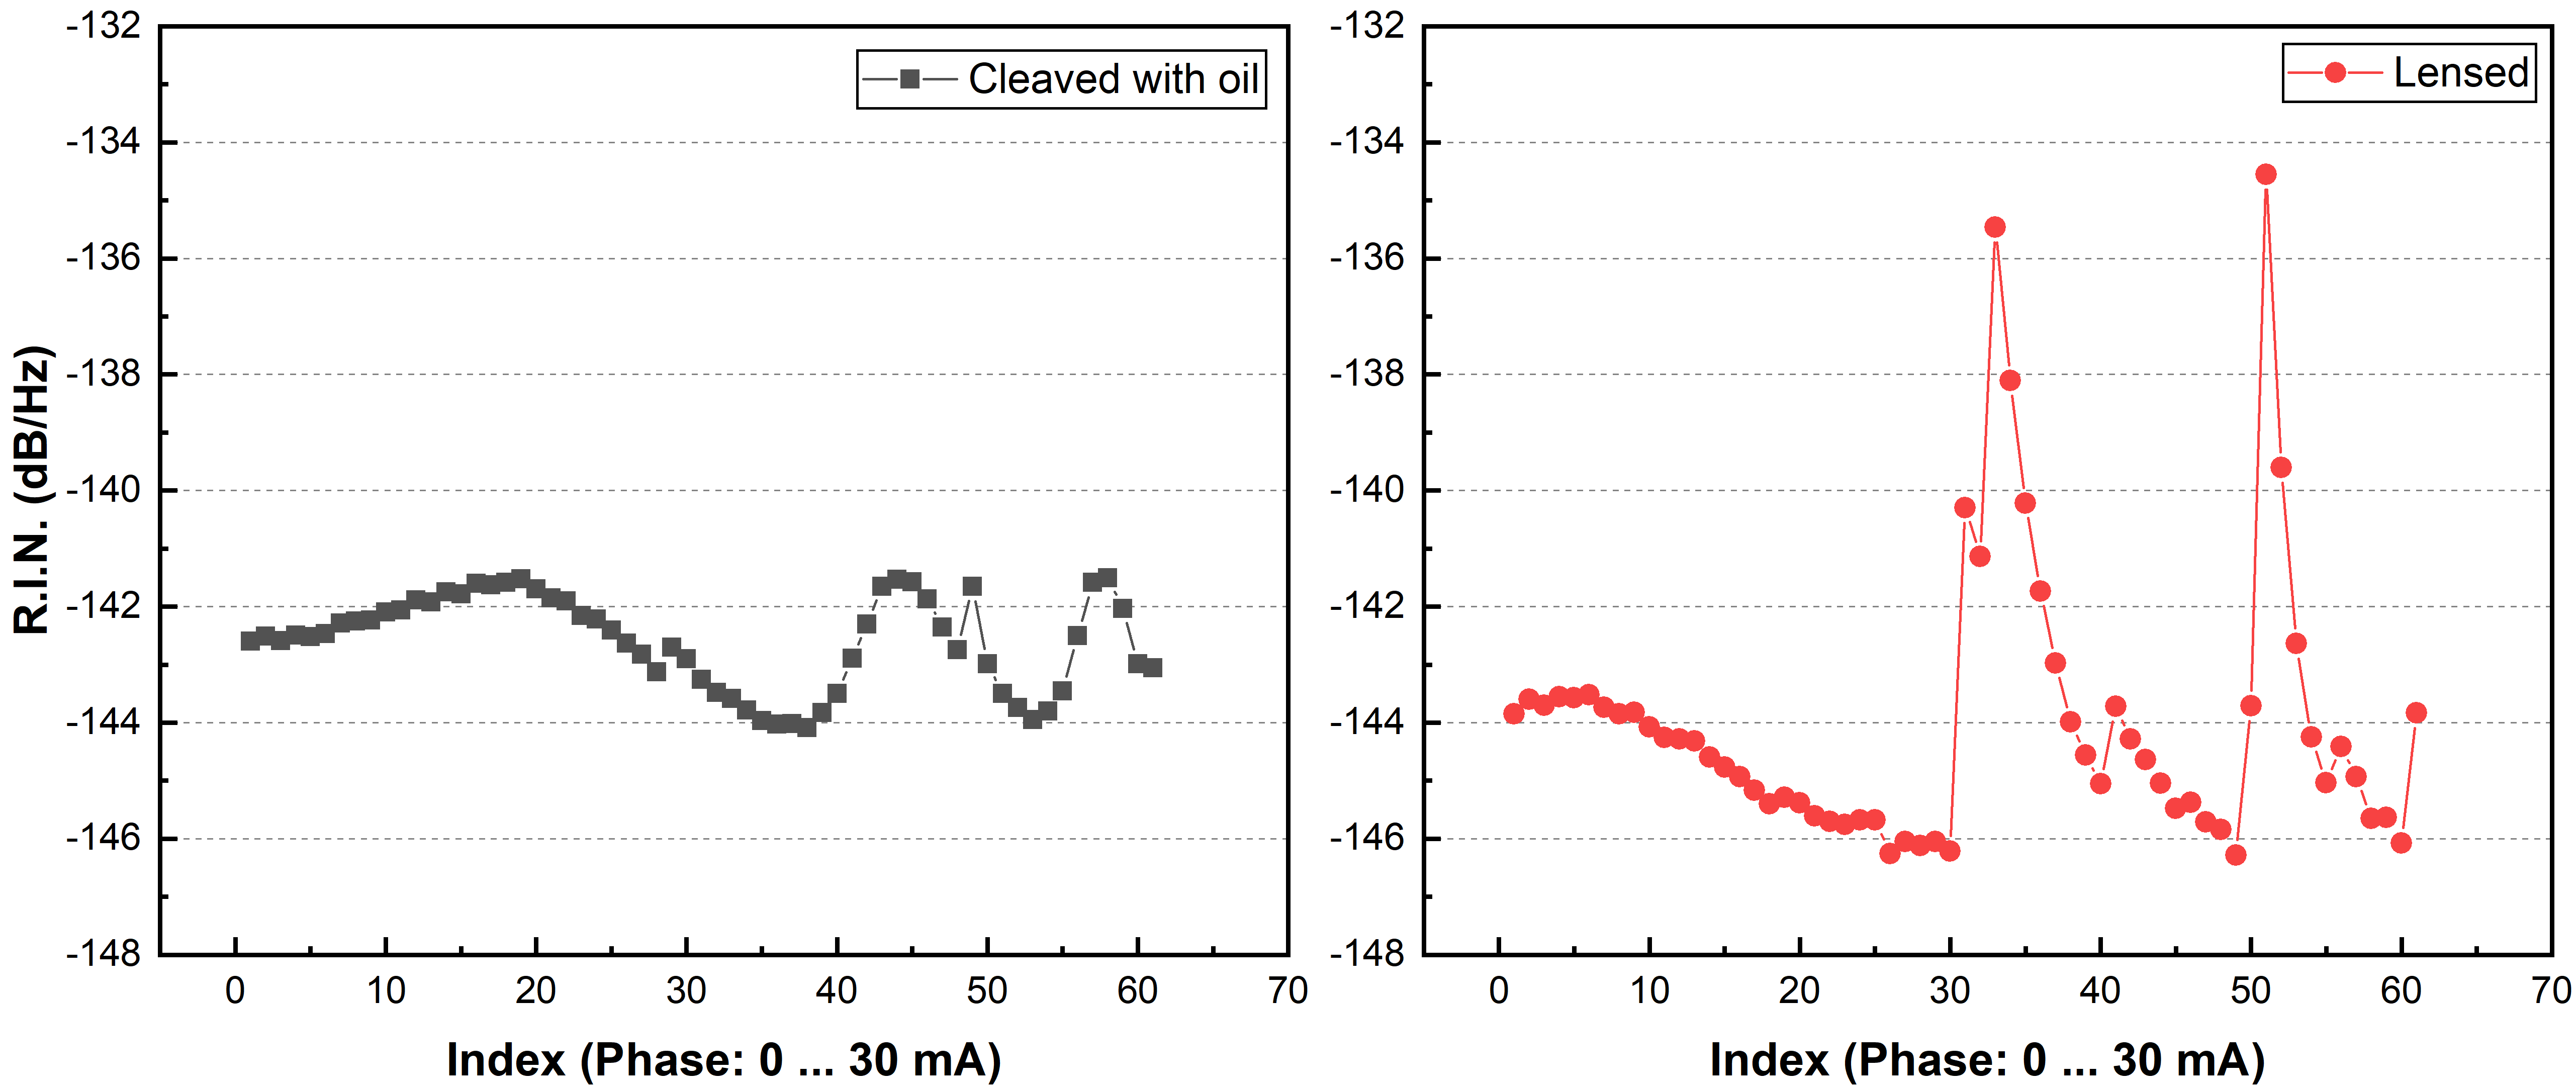
\includegraphics[width=\linewidth]{figures/RIN_cleaved_and_lensed.png}
    \caption{Caption}
    \label{fig:RIN_cleaved_and_lensed}
\end{figure}

\section{Bandwidth Measurement}\label{sec:bandwidth_measurement}
\subsection{Small Signal Modulation}
From a practical viewpoint the quantity of interest is the modulation bandwidth $\nu_B$ which indicates the frequency range over which the laser responds to the current modulation. It is usually defined as the frequency at which the modulation response has dropped by 3 dB relative to its low-frequency or DC value \cite{agrawal2013semiconductor}.
\begin{figure}[ht]
    \centering
    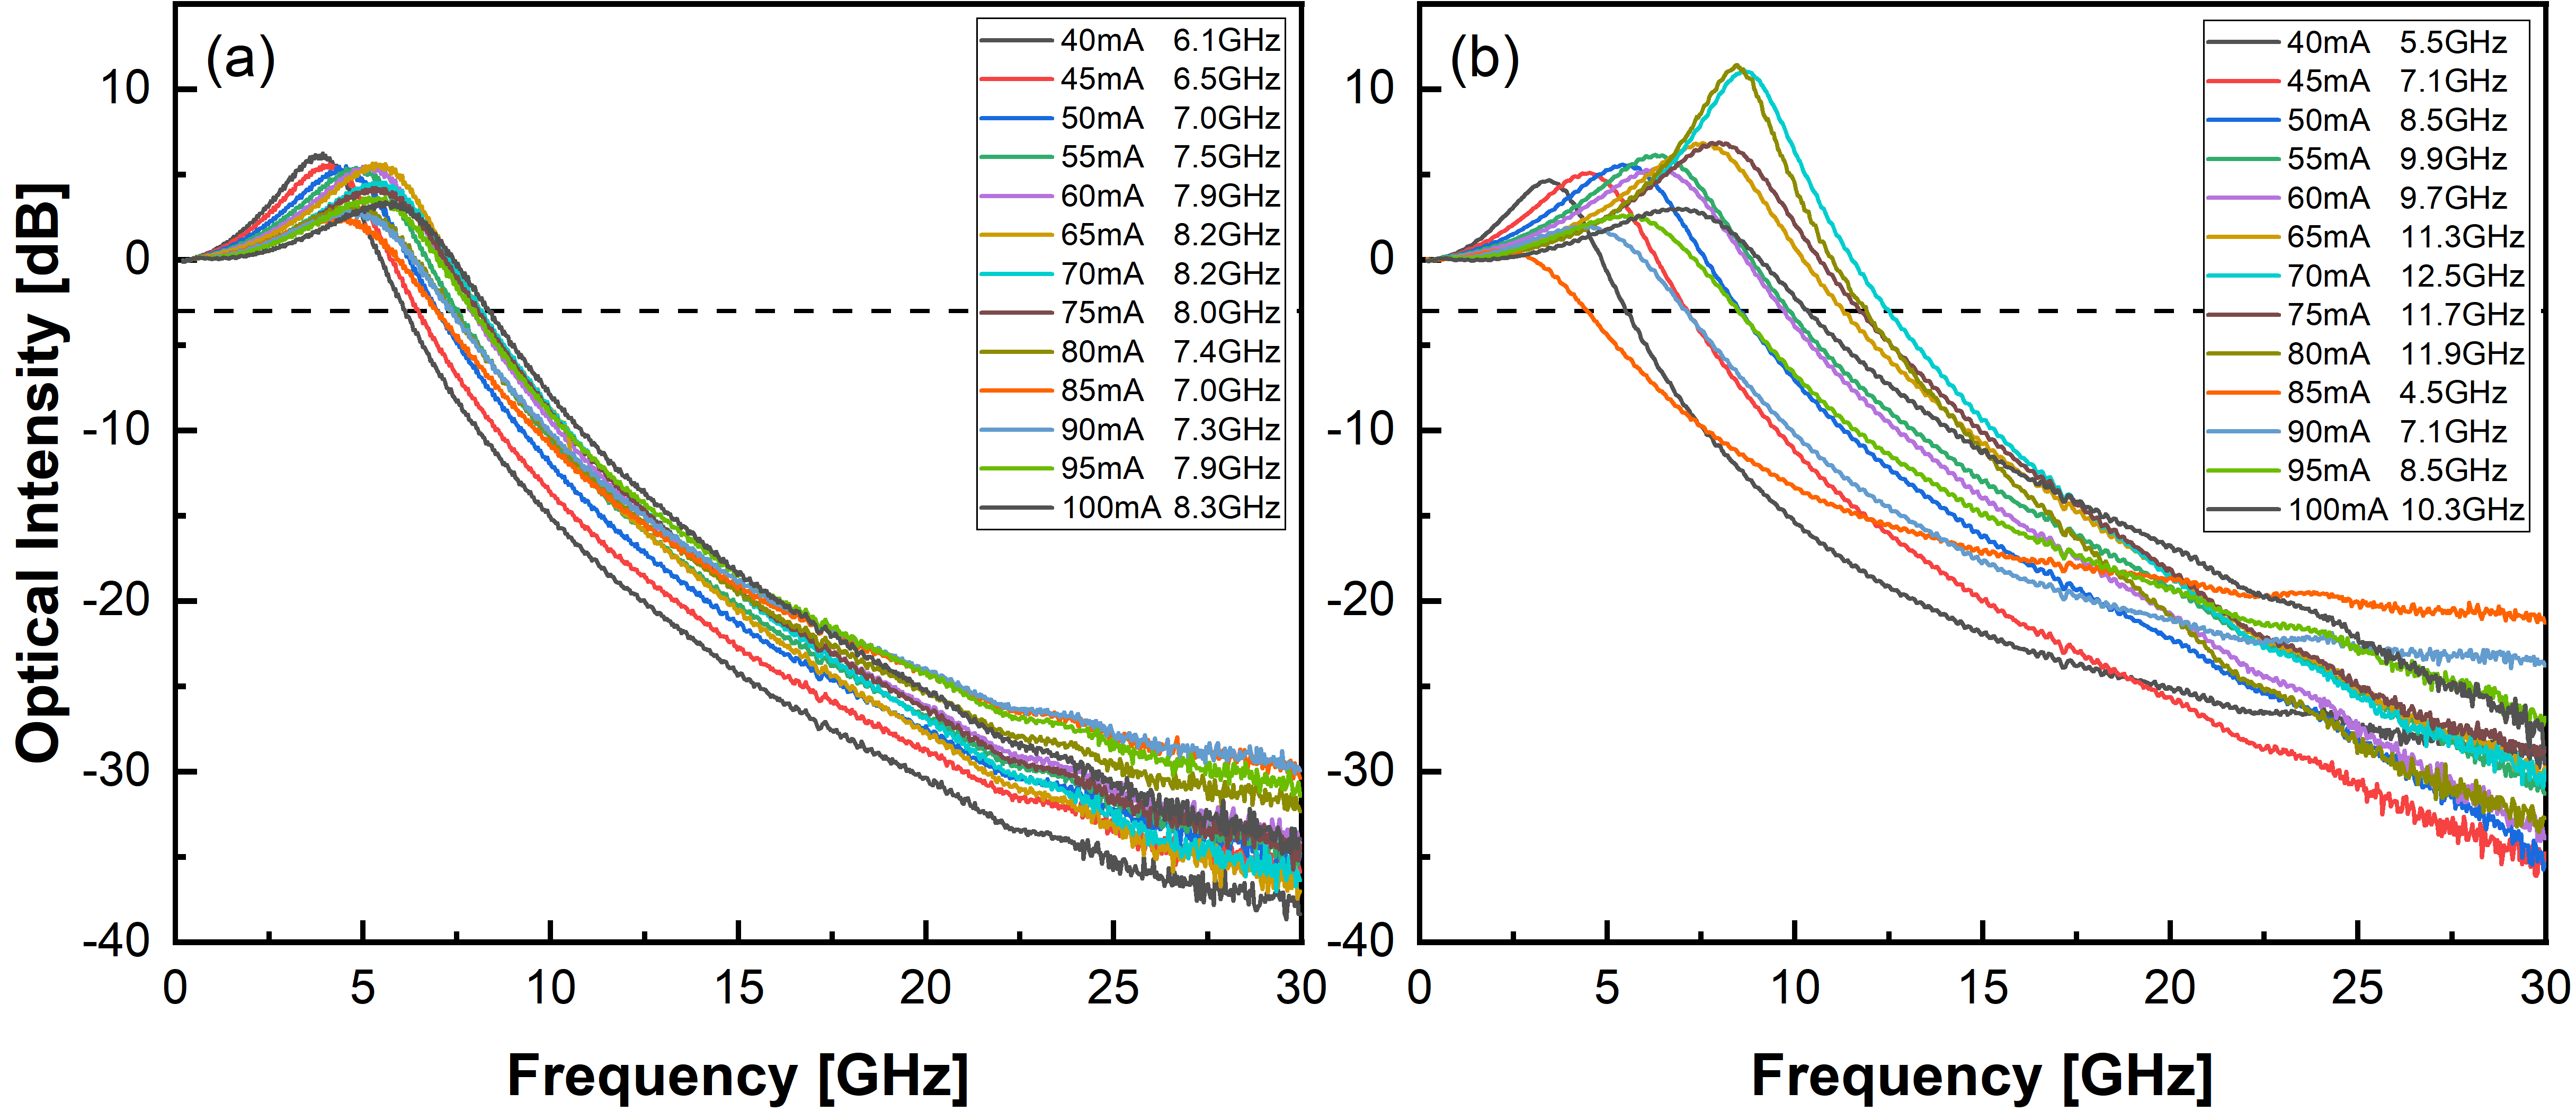
\includegraphics[width=\linewidth]{figures/bandwidth_gain_scan_cleaved_and_lensed_grating_4679.png}
    \caption{Caption}
    \label{fig:bandwidth_gain_scan_cleaved_and_lensed}
\end{figure}

The frequency response of the laser transmitter under small signal modulation is found by the usual assumption of a harmonic current modulation superimposed on a constant bias above threshold.
\begin{equation}
    H(\omega)=\frac{\omega_R^2}{\omega_R^2-\omega^2-2j\omega\gamma}
    \label{modulation_transfer_function}
\end{equation}
in \autoref{modulation_transfer_function}, $\omega_R$ is the relaxation resonance frequency and $\gamma$ is the damping factor.

The relaxation oscillation frequency is a measure of the maximum modulation ability in semiconductor lasers through the injection current. Above the relaxation oscillation, the modulation efficiency is greatly degraded and intensity modulation through the injection current becomes difficult. [Semiconductor Lasers. Stability, Instability and Chaos.pdf]

\textit{The laser seeks a steady-state operation which maximizes feedback. When external feedback is present, the state corresponding to maximum feedback occurs when there is phase alignment  between the semiconductor cavity field and the reflected field. A carrier number change $n$ will change the resonance frequency of the semiconductor cavity. This in turn causes a phase change $\phi$ between the laser field and the reflected field. This acts to decrease the light intensity in proportion to $1-cos{\phi}\approx\frac{\phi^2}{2}$, which decreases the rate of stimulated emission and further increases $n$. This increase in $n$ again raises the cavity resonance frequency, causing the phase misalignment $\phi$ to continue to grow. Instability occurs for finite fluctuations of $\phi$ and $n$ when this effect becomes greater than the restoring forces giving rise to the relaxation oscillations described above.}

\textit{steady-state operation (phase alignment of the cavity field and reflected field)}

\textit{In steady-state operation, the laser with reflective feedback can be thought of as phase locked to the reflected field. The phenomenon that we describe is driven by large fluctuations in spontaneous emission that dislodge the laser from this locked state that is stable for small fluctuations. [Henry, Kazarinov 1986]}

\subsubsection{Detuend loading condition}
\begin{figure}[!htb]
    \centering
    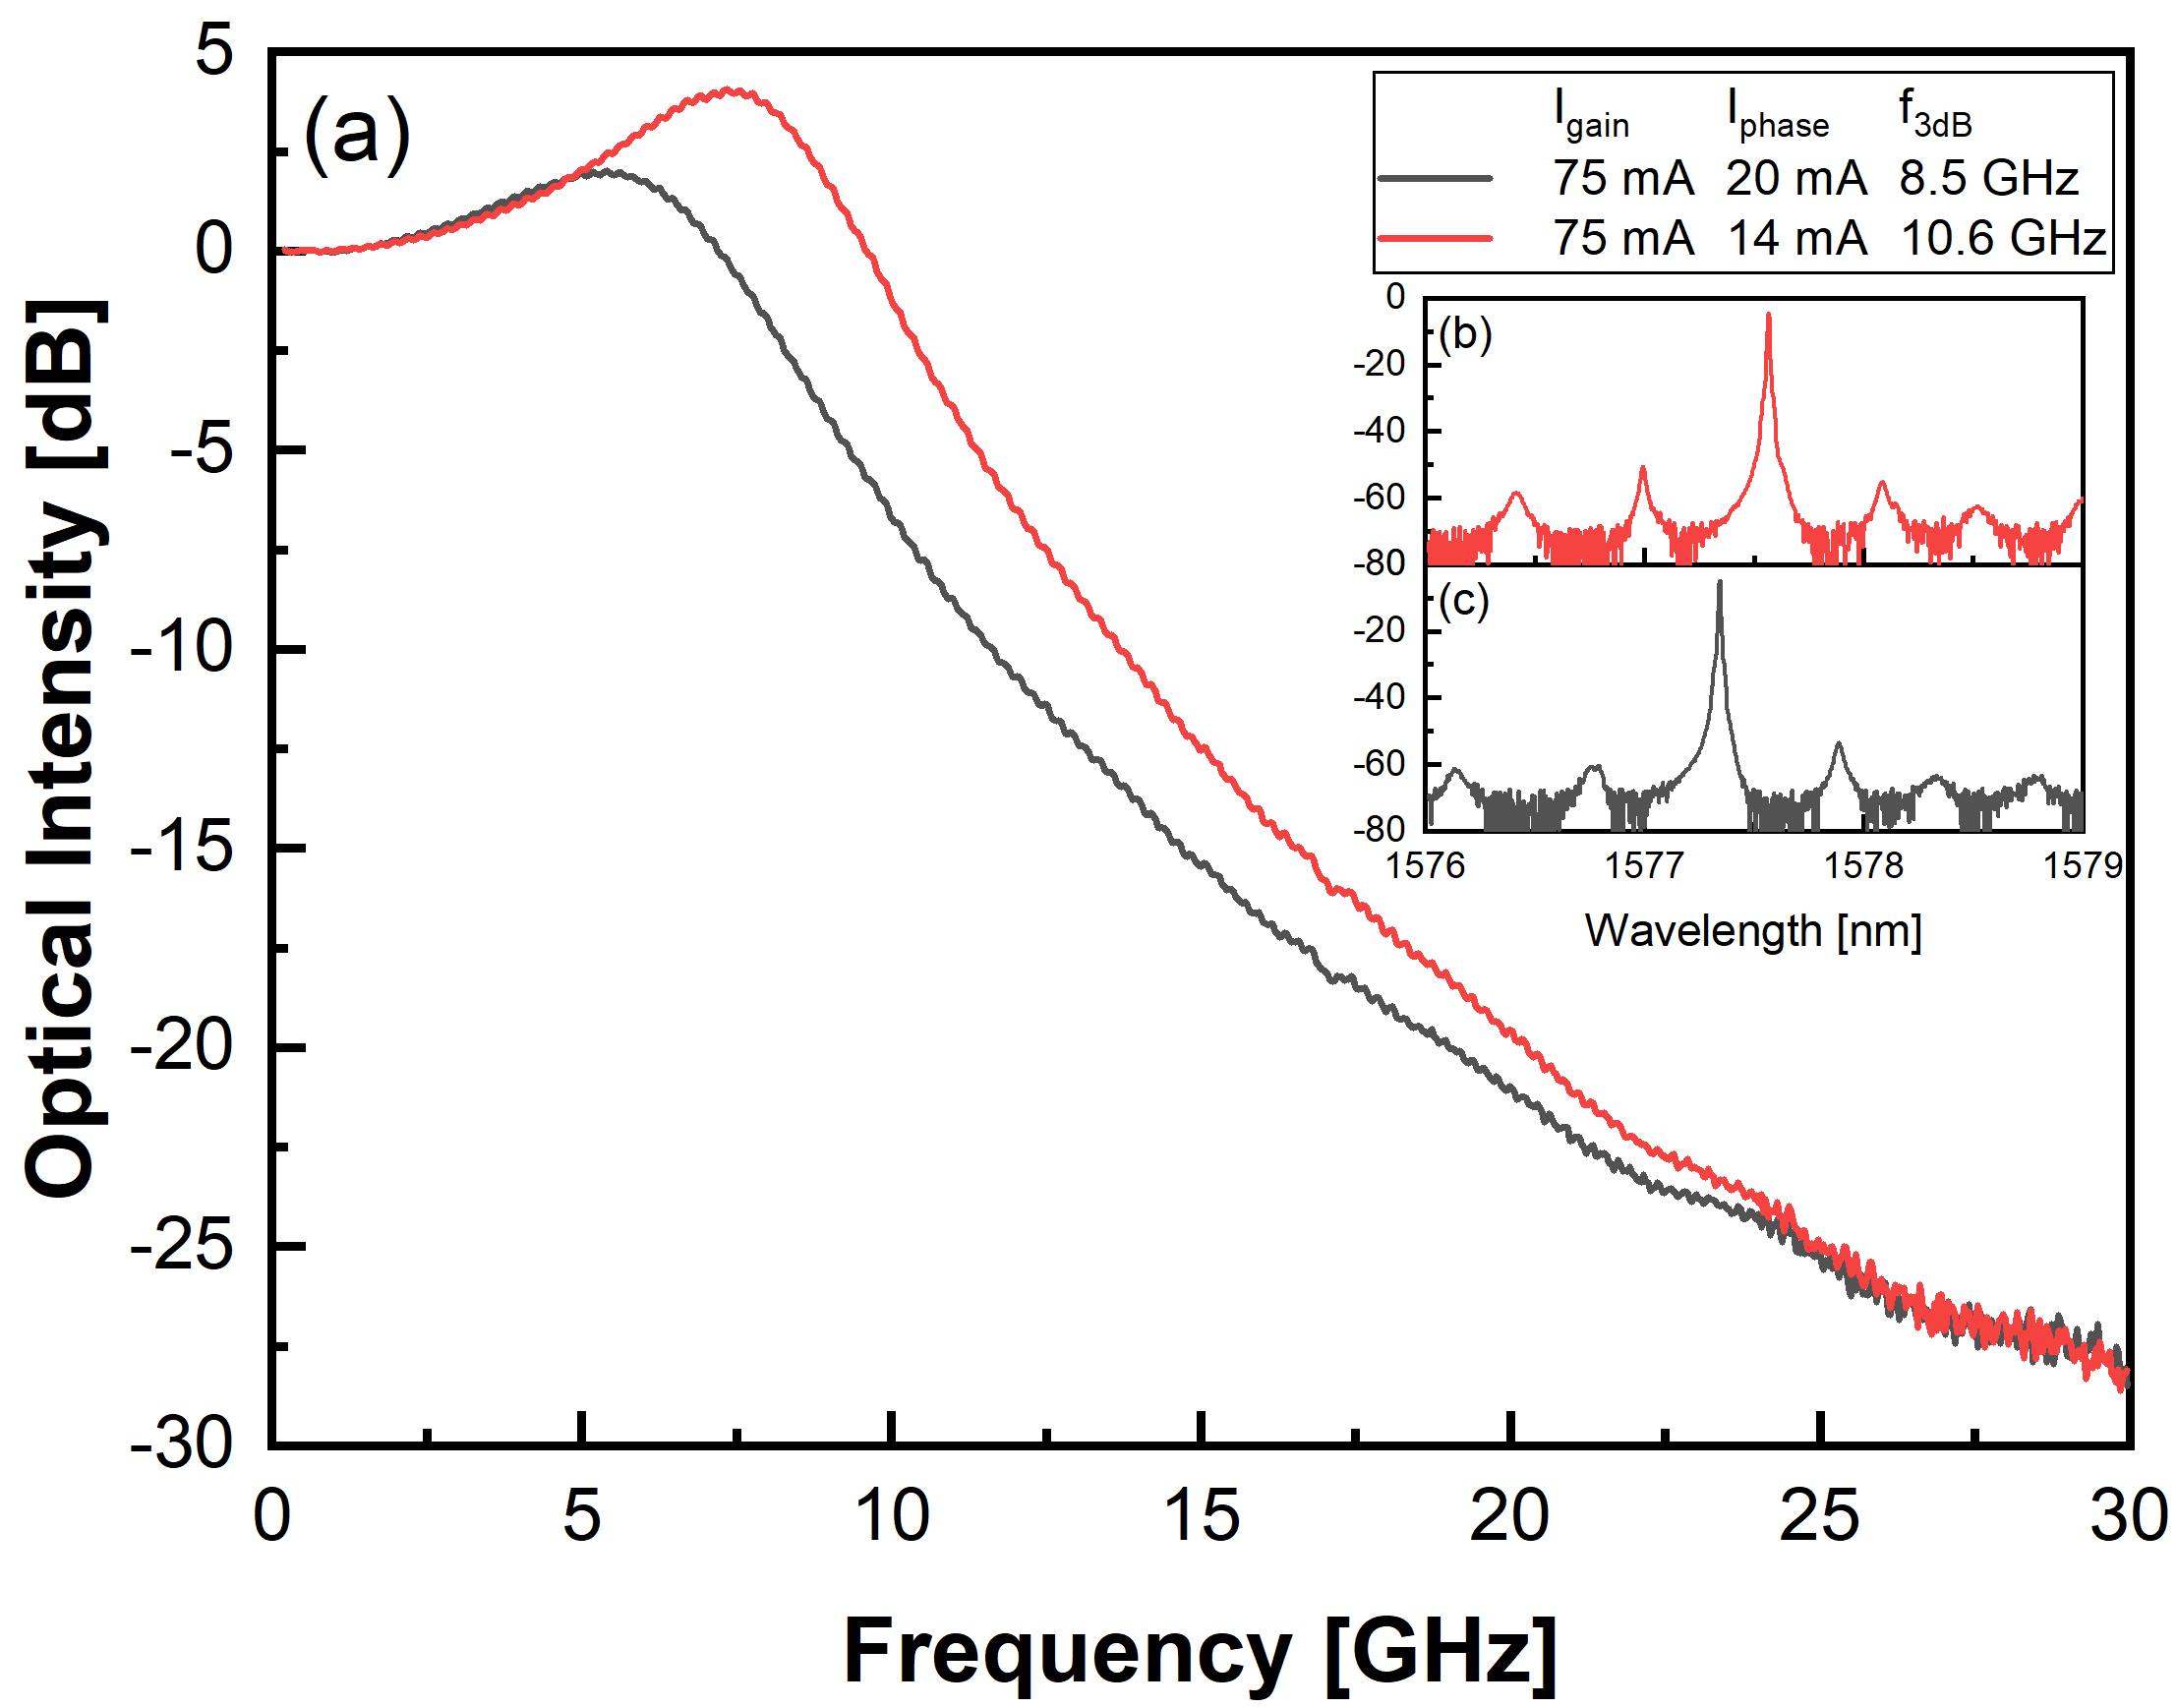
\includegraphics[width=.6\linewidth]{figures/detuned_loading.png}
    \caption{Bandwidth enhancement with the detuned loading condition on our tunable laser device. The red curve is detuned to the longer wavelength side of the grating response, shows an increased bandwidth of 2.1 GHz compared to the grey curve without bandwidth enhancement effect.}
    \label{fig:detuned_loading}
\end{figure}

\subsubsection{Undamped RO}
\begin{figure}[!htb]
    \centering
    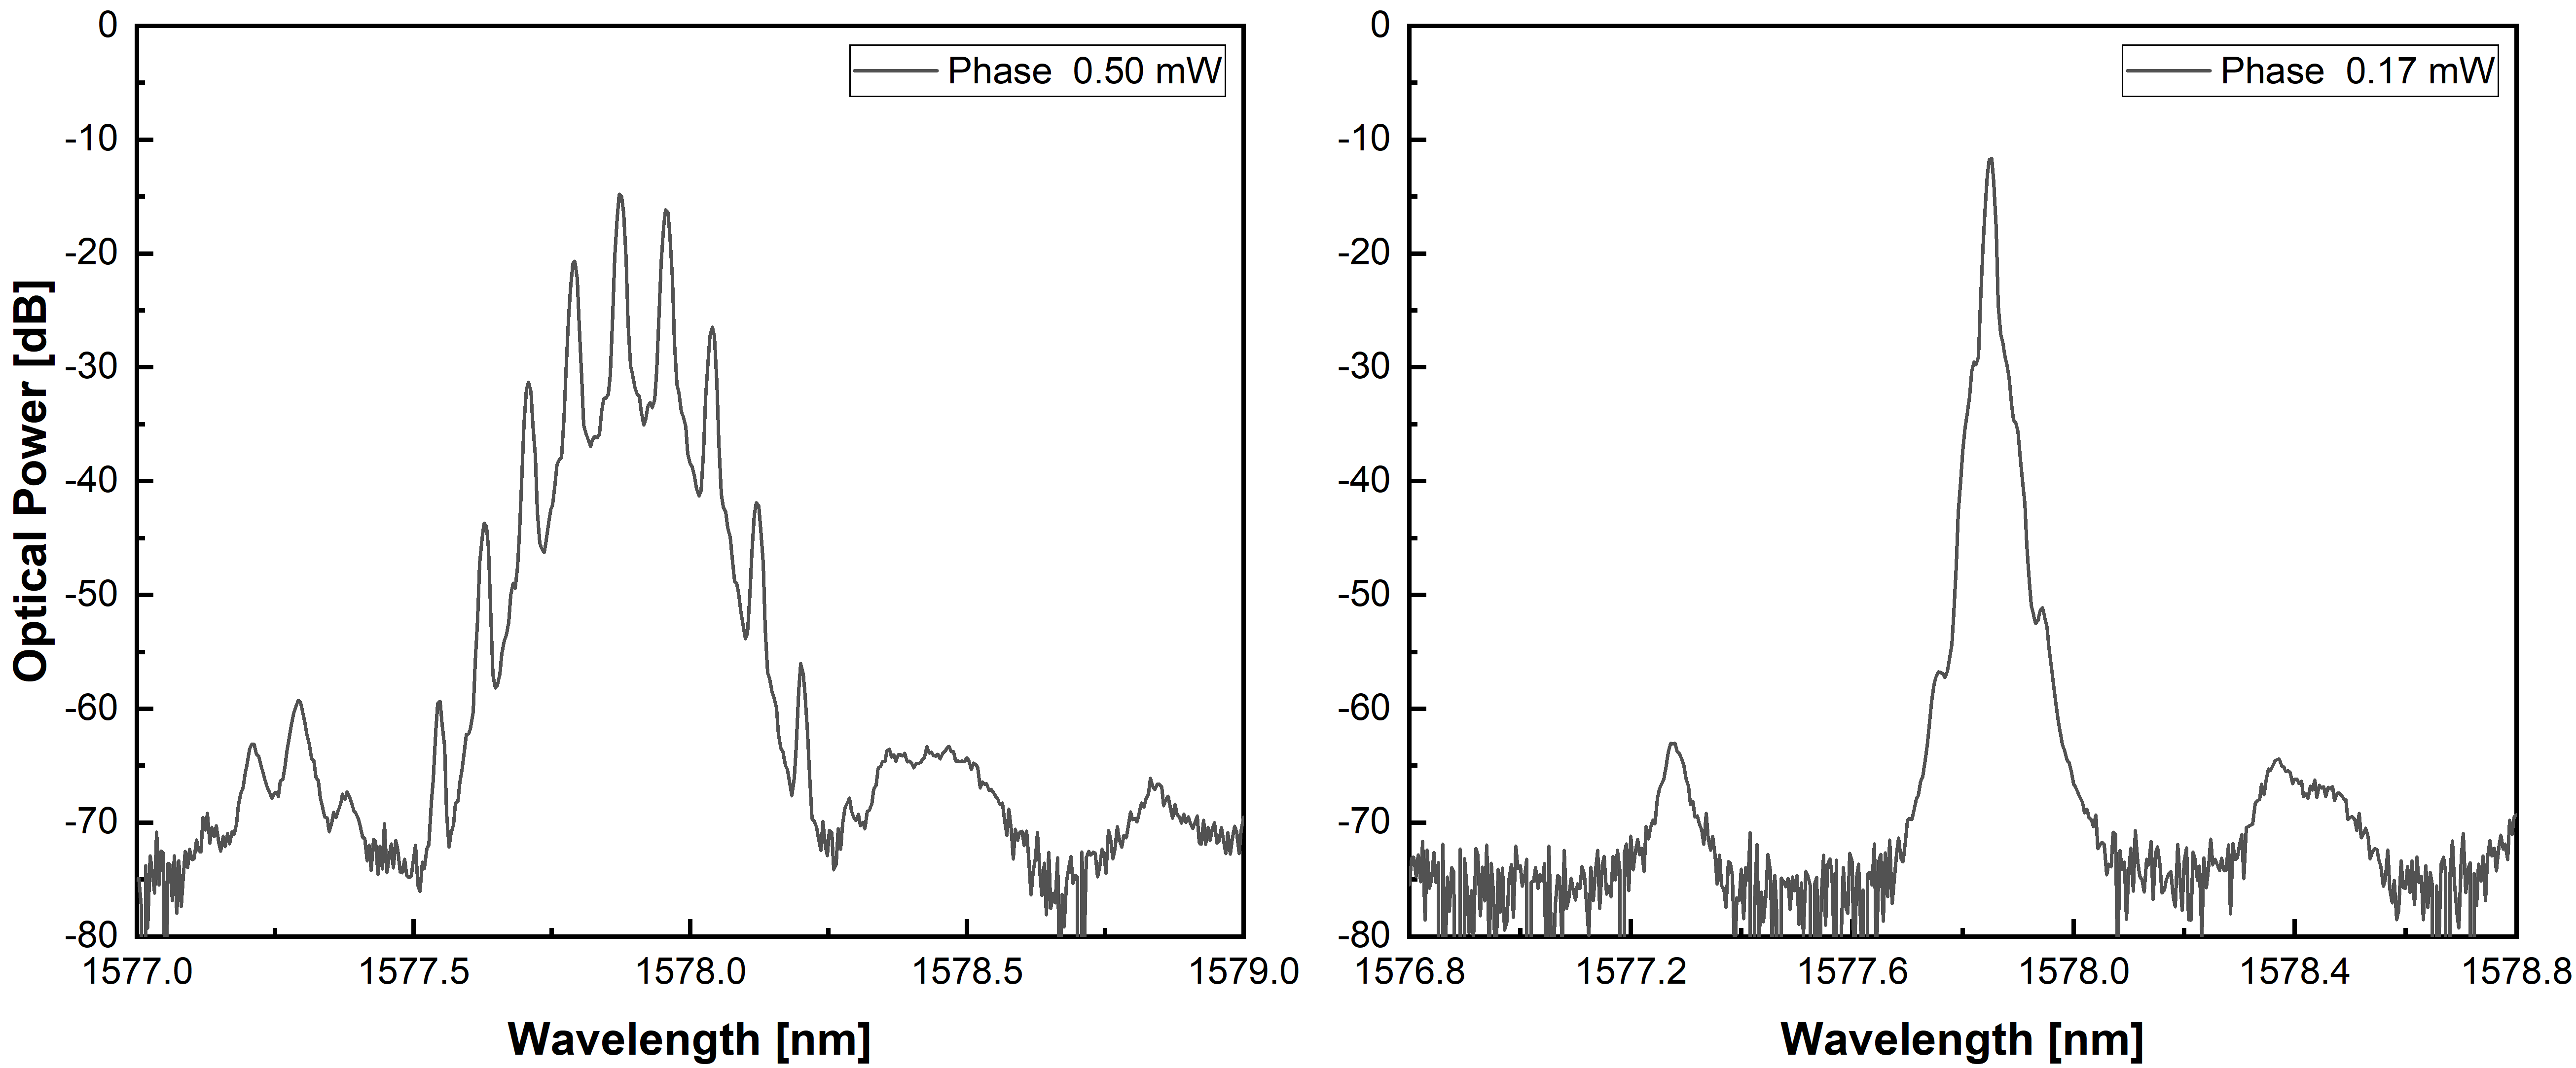
\includegraphics[width=.9\linewidth]{figures/Undamped_RO_grating_4621.png}
    \caption{Observation of the undamped relaxation oscillation in OSA.}
    \label{fig:undamped_RO}
\end{figure}

\subsection{}
\textit{Chirp arises because the frequency of the laser mode depends on the carrier number in the active region. Above threshold, the carrier number changes because of two effects: spectral hole burning prohibits the perfect pinning of the carrier number and permits adiabatic chirp, and during transients, there are relaxation oscillations of carrier number, which cause dynamic chirp. [Kazarinov 1987]}

\textit{Current modulation of the active region results in a modulation of both the photon density and the carrier density. The modulation of the carrier density modulates the gain; however, it also modulates the index of the active region na . As a result, the optical length of the cavity is modulated by the current, causing the resonant mode to shift back and forth in frequency. [Larry A. Coldren.pdf]}

If we consider the case discussed earlier where the semiconductor cavity is extended by a passive section of length $L_1$, with a nonreflective transition between the two sections, the reflection at the semiconductor section constant in magnitude, but has a frequency-dependent phase shift with $d\phi_r/d\omega = 2L_1/v_g1$ where $2L/v_g1$ is the roundtrip time in the external cavity. Therefore, in this case $B=0$, the chirp reduction factor is [Kazarinov 1987]



\section{Chirp Parameter ($\alpha$-Factor) Measurement}
Light chirping is a parasitic property of intensity modulated light. It originates in light emitters that produce a phase shift as the intensity is varied \cite{devaux1993simple}. Semiconductor lasers exhibit a particular nonlinearity in the interaction of the light with the active medium, which distinguishes them from all other lasers. The nonlinearity originates from the physics of the semiconductor band structure, since the photon generation typically occurs due to interband transitions. The gain spectrum of such lasers therefore does not exhibit a symmetric peak, as atomic transitions do, but has a strongly asymmetric shape. This affects the dispersive properties of the lasers as well, since those properties are connected via the Kramers-Kronig relation. As a consequence, the dispersion curve for the refractive index exhibits its zero crossing at higher frequency than the maximum of the gain spectrum. If the gain changes, e.g., by a change of the carrier density, the refractive index changes as well, which would not be the case for atomic transitions. Hence, changes in gain are in semiconductor lasers associated with changes in refractive index and vice versa. Since with a change of refractive index of the medium the optical frequency and thus the optical phase changes, one also speaks of amplitude phase coupling. A small change in the intensity (induced, e.g., by a change in the injection current, by dynamical instabilities, or even a spontaneous emission event) causes an excess perturbation of the phase of the lasing mode. In the rate equation description, the effect is taken into account via the so-called $\alpha$ parameter, which is also referred to as Henry parameter or linewidth enhancement factor. It is defined as
\begin{equation}
    \alpha=-\frac{\dv*{\chi_r(n)}{n}}{\dv*{\chi_i(n)}{n}}
\end{equation}

\subsection{Measurement with LCA}\label{subsec:measurement_with_LCA}
The network analyzer of \autoref{fig:LCA_setup} measures the small-signal frequency response of a light emitter, a dispersive medium and a light receiver. The dispersive medium is 81 $km$ of standard, single-mode fiber (zero dispersion at 1.3 $\mu m$) from and Er-doped fiber amplifiers pumped at 1.55 $\mu m$. Resonance frequencies are observed as sharp peaks in the frequency response.
\begin{figure}[ht]
    \centering
    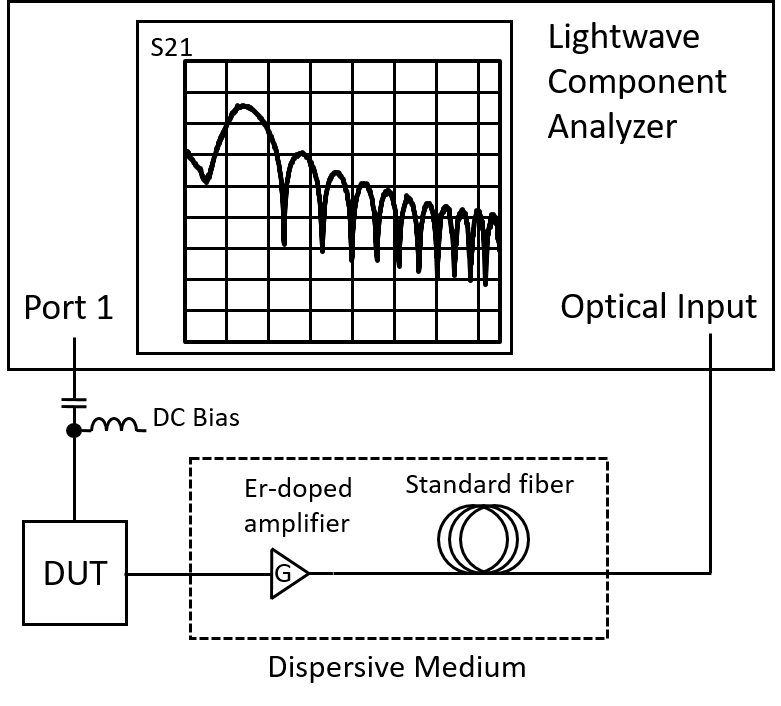
\includegraphics[width=.5\linewidth]{figures/LCA_setup.png}
    \caption{Set-up used to measure the chirp parameter of the laser}
    \label{fig:LCA_setup}
\end{figure}

The resonance frequencies $f_u$ of Fig.2 corresponds to the $u^{th}$-zeros of xx. They follow a very simple law:
\begin{equation}
    f_u^2L=\frac{c}{2D\lambda ^2}(1+2u-\frac{2}{\pi}arctan(\alpha))
    \label{eq:LCA_equa}
\end{equation}

The equation is the result of two simultaneous interferences between the carrier and the two sidebands. Plotting $f_u^2L$ versus $2u$ gives a straight line whose slope and position yield the dispersion and the chirp parameter by liner regression.

\subsection{AM-FM Index Method}
The experimental arrangement for measuring the intensity and phase modulation index is shown in Fig. 1. The semiconductor laser is biased above threshold and a small sinusoidally varying current at frequency $\Omega$ is superimposed. The intensity and spectral density of the radiation field are given by
\begin{equation}
    Intensity: E_0^2[1+mcos(\Omega t)]
\end{equation}
\begin{equation}
    Spectrum: Center \ line \ at \ \omega_1: E_0^2[J_0^2(\beta)+m^2J_1^2(\beta)]
    \label{eq:alpha_2}
\end{equation}
\begin{equation}
    First \ sidebands \ at \
    \ \omega_1 \pm \Omega: E_0^2\big\{J_1^2(\beta)+1[(m/2)(J_2(\beta)-J_0(\beta))]^2\big\}
    \label{eq:alpha_3}
\end{equation}

The phase modulation index $\beta$ can be found by measuring the relative sideband strength and using \autoref{eq:alpha_2} and \autoref{eq:alpha_3}. The factor $\alpha_m$ is then obtained as $\alpha_m = -2(\beta/m)$.
\begin{figure}[ht]
    \centering
    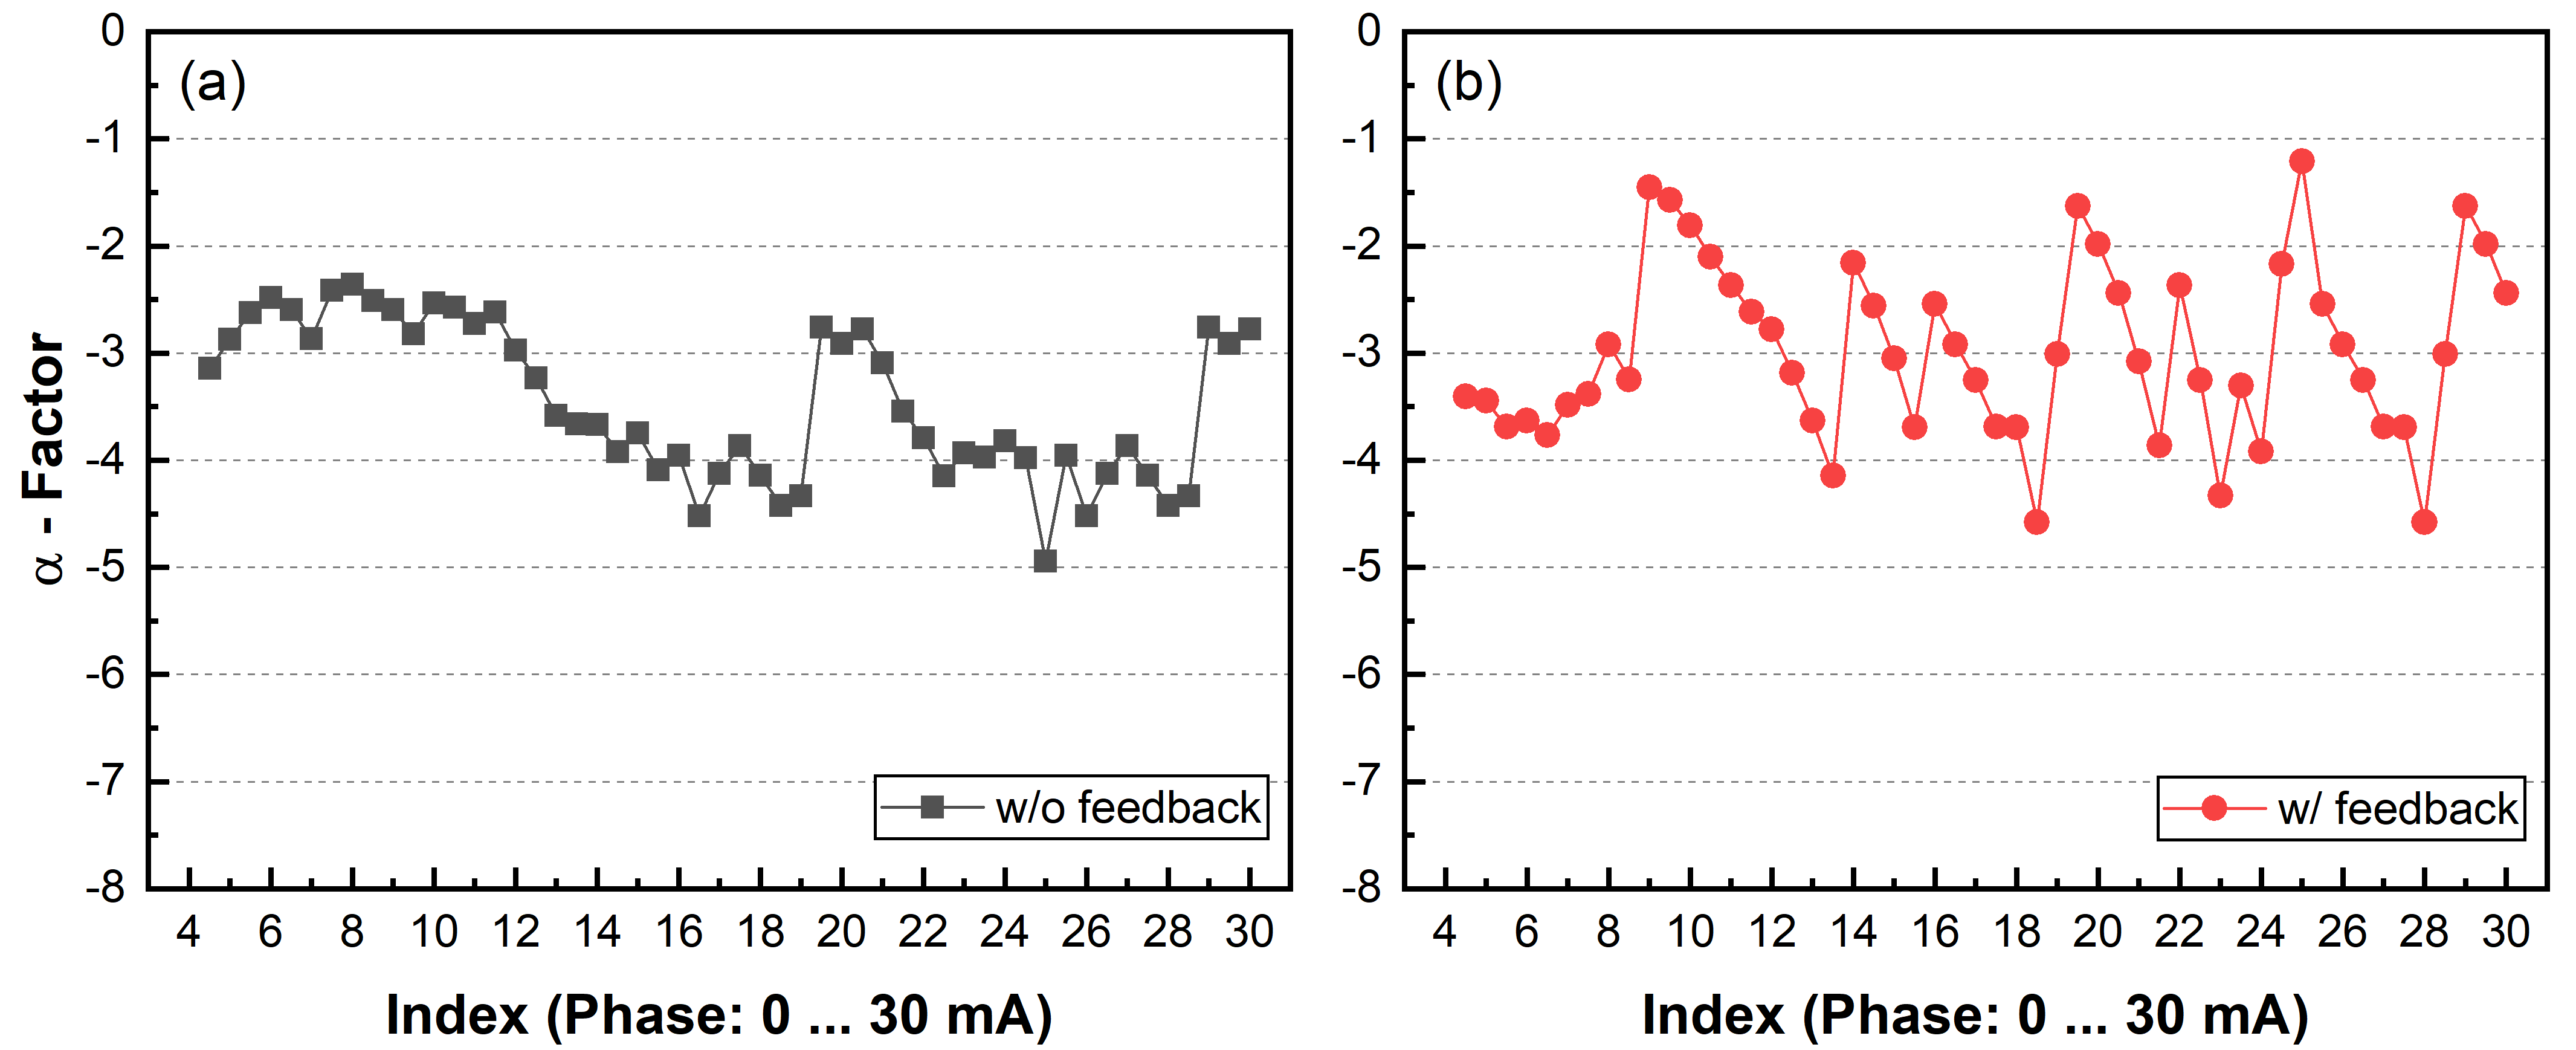
\includegraphics[width=\linewidth]{figures/Alpha_Cleaved_and_Lensed.png}
    \caption{Comparison of $\alpha$ parameter}
    \label{fig:Alpha_Cleaved_and_Lensed}
\end{figure}

\section{Phase Noise Measurement}

